%==================================================================================================
\section{Estudo numéricos de escoamentos incompressíveis} \label{ExemplosMT}
%==================================================================================================

Para verificação e estudo das características numéricas das formulações implementadas para a mecânica dos fluidos, são realizadas simulações de problemas cuja solução é bem estabelecida na literatura, adotando tanto com discretizações bidimensionais quanto tridimensionais. Inicia-se com o estudo de problemas com contornos fixos (velocidade da malha nula em todo o domínio), e posteriormente, simula-se também dois exemplos com contornos móveis.

%==================================================================================================
\subsection{Cavidade bidimensional} \label{ex:cavity}
%==================================================================================================

Este problema é comumente utilizado na literatura como \textit{benchmark} para verificação de formulações numéricas para escoamentos incompressíveis, tratando-se de uma cavidade quadrada com paredes aderentes, onde o fluido encontra-se confinado e sujeito a uma velocidade horizontal prescrita $\BB{u}_\infty$ no topo devida ao deslizamento da parede, como apresentado na Figura \ref{fig:cavity}. Devido ao fato do problema possuir apenas fronteiras de Dirichlet, o condicionamento da solução do campo de pressão é garantido pela aplicação de uma condição de pressão nula no centro da aresta inferior da cavidade. Também se observa que existe uma descontinuidade nas condições de contorno no encontro entre as paredes laterais da cavidade e o topo, podendo ser consideradas velocidades nulas ou igual à velocidade do topo. No problema em questão considerou-se que a velocidade nesse ponto é igual à $\BB{u}_\infty$.

\begin{figure}[h!]
    \centering
    \caption{Cavidade bidimensional - Desenho esquemático}
    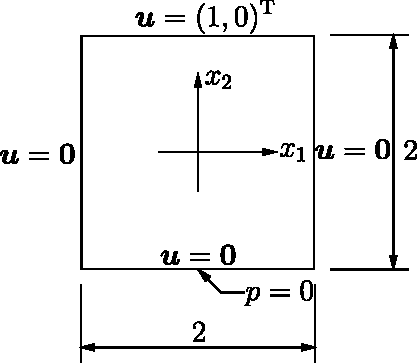
\includegraphics[width=.4\linewidth]{Figuras/Cavity/cavidade.pdf}
    \\Fonte: Presente trabalho (\the\year).
    \label{fig:cavity}
\end{figure}.

Considera-se o fluido com densidade unitária $\rho=1,0$ e velocidade no topo também unitária para todas as análises, enquanto a viscosidade do fluido é modificada para obter-se diferentes números de Reynolds. São considerados os casos com número de Reynolds 100, 400, 1.000, 5.000, 7.500 e 10.000, tomando o lado da cavidade como comprimento característico. O problema parte do repouso em todas as simulações, sendo considerado o passo de tempo $\Delta t=0,1$ com $\rhoinf=0,0$ para o integrador temporal, sendo a simulação mantida até que a estacionariedade fosse alcançada.

Inicialmente são empregadas 3 diferentes discretizações bidimensionais, uma com elementos triangulares de aproximação quadrática tanto para velocidade quanto para pressão, outra com elementos triangulares Taylor-Hood de aproximação quadrática para velocidade e linear para pressão (P2P1), e uma terceira com elementos triangulares de aproximação linear tanto para velocidade como para pressão, conforme as características apresentadas na tabela \ref{tab:cavity-mesh}, onde $n_u$ e $n_p$ são os números de nós para interpolação dos campos de velocidade e de pressão, respectivamente. Essas malhas são ilustradas na figura \ref{fig:cavity-mesh}.

\begin{table}[h!]
    \centering
    \caption{Cavidade bidimensional - Características das malhas utilizadas.}
    \begin{tabular}{lcccc}
        \hline
        Malha & Elementos & $n_u$ & $n_p$ & DOF   \\\hline
        P1P1  & 12800     & 6561  & 6561  & 19683 \\
        P2P2  & 3200      & 6561  & 6561  & 19683 \\
        P2P1  & 3200      & 6561  & 1681  & 14803 \\\hline
    \end{tabular}
    \\Fonte: Presente trabalho (\the\year).
    \label{tab:cavity-mesh}
\end{table}

\begin{figure}[h!]
    \centering
    \caption{Cavidade bidimensional - Malhas utilizadas.}
    \begin{subfigure}{0.49\textwidth}
        \centering
        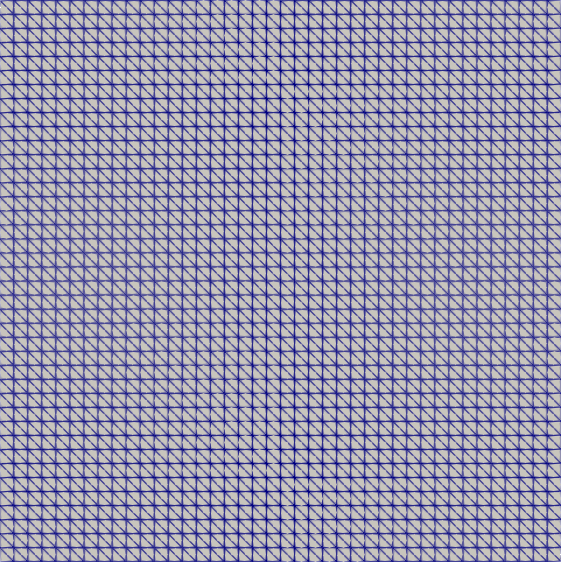
\includegraphics[width=.8\linewidth]{Figuras/Cavity/m1.png}
        \caption{Malha de elementos P2P2 e P2P1.}
    \end{subfigure}
    \begin{subfigure}{0.49\textwidth}
        \centering
        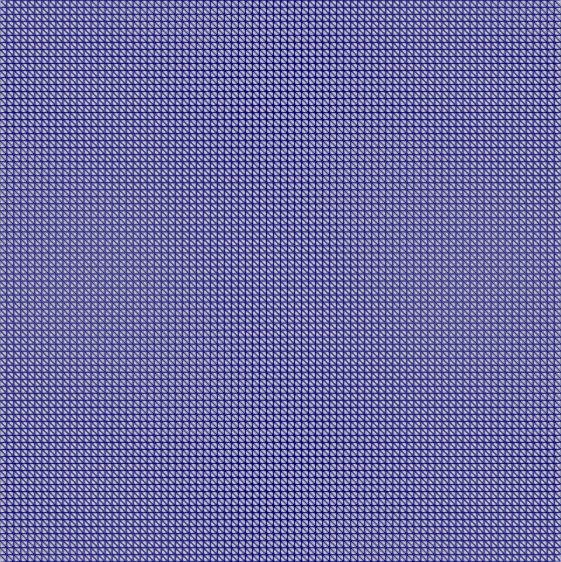
\includegraphics[width=.8\linewidth]{Figuras/Cavity/m1-Lin.png}
        \caption{Malha de elementos P1P1.}
    \end{subfigure}
    \\Fonte: Presente trabalho (\the\year).
    \label{fig:cavity-mesh}
\end{figure}

Assim, para cada número de Reynolds as simulações são realizadas considerando-se: 1) elementos finitos P1P1 com estabilização SUPG/PSPG; 2) elementos P2P2 com estabilização por SUPG/PSPG; 3) elementos P2P2 com formulação VMS; 4) elementos P2P1 estabilizados por SUPG, e 4) a combinação de cada um dos casos anteriores com o modelo de turbulência LES, adotando-se constante de Smagorinsky $C_S=0,10$.


A Figura \ref{fig:cavity-results} apresenta os valores obtidos para velocidades sobre as linhas médias da cavidade ($y_1=0$ e $y_2=0$) por cada uma das simulações, comparando-se os resultados obtidos com aqueles apresentados por \citeonline{ghia1982high}.

\begin{figure}[h!]
    \centering
    \caption{Cavidade bidimensional - distribuição de velocidade sobre as linhas médias.}
    \begin{subfigure}{0.4\textwidth}
        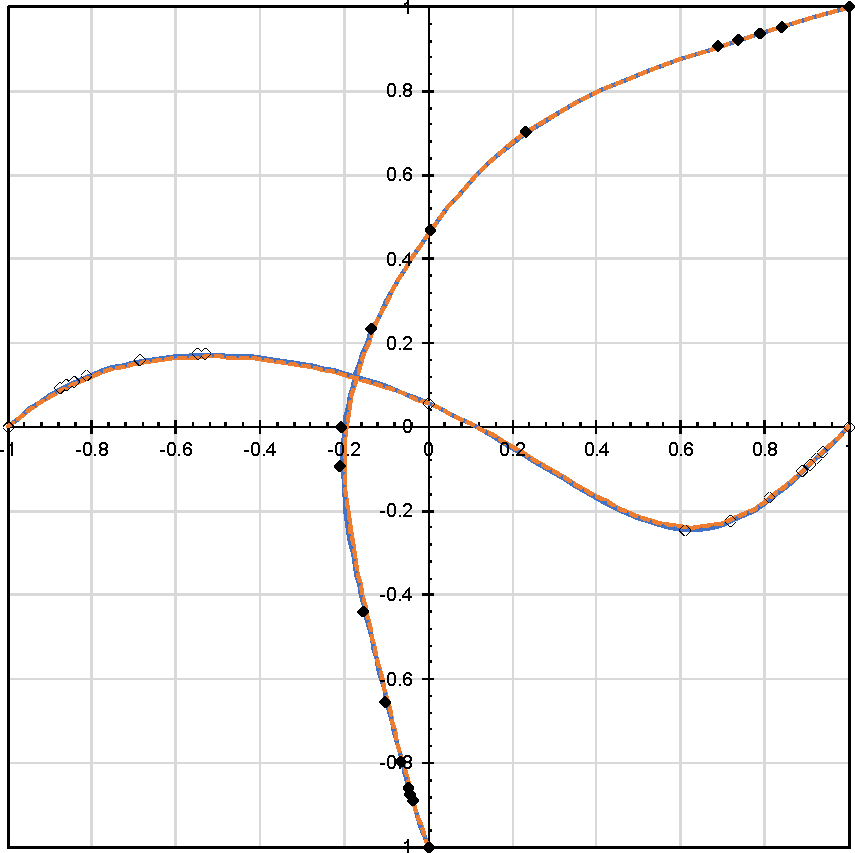
\includegraphics[width=\linewidth]{Figuras/Cavity/Re100.pdf}
        \caption{$\Rey=100$}
    \end{subfigure}
    \begin{subfigure}{0.4\textwidth}
        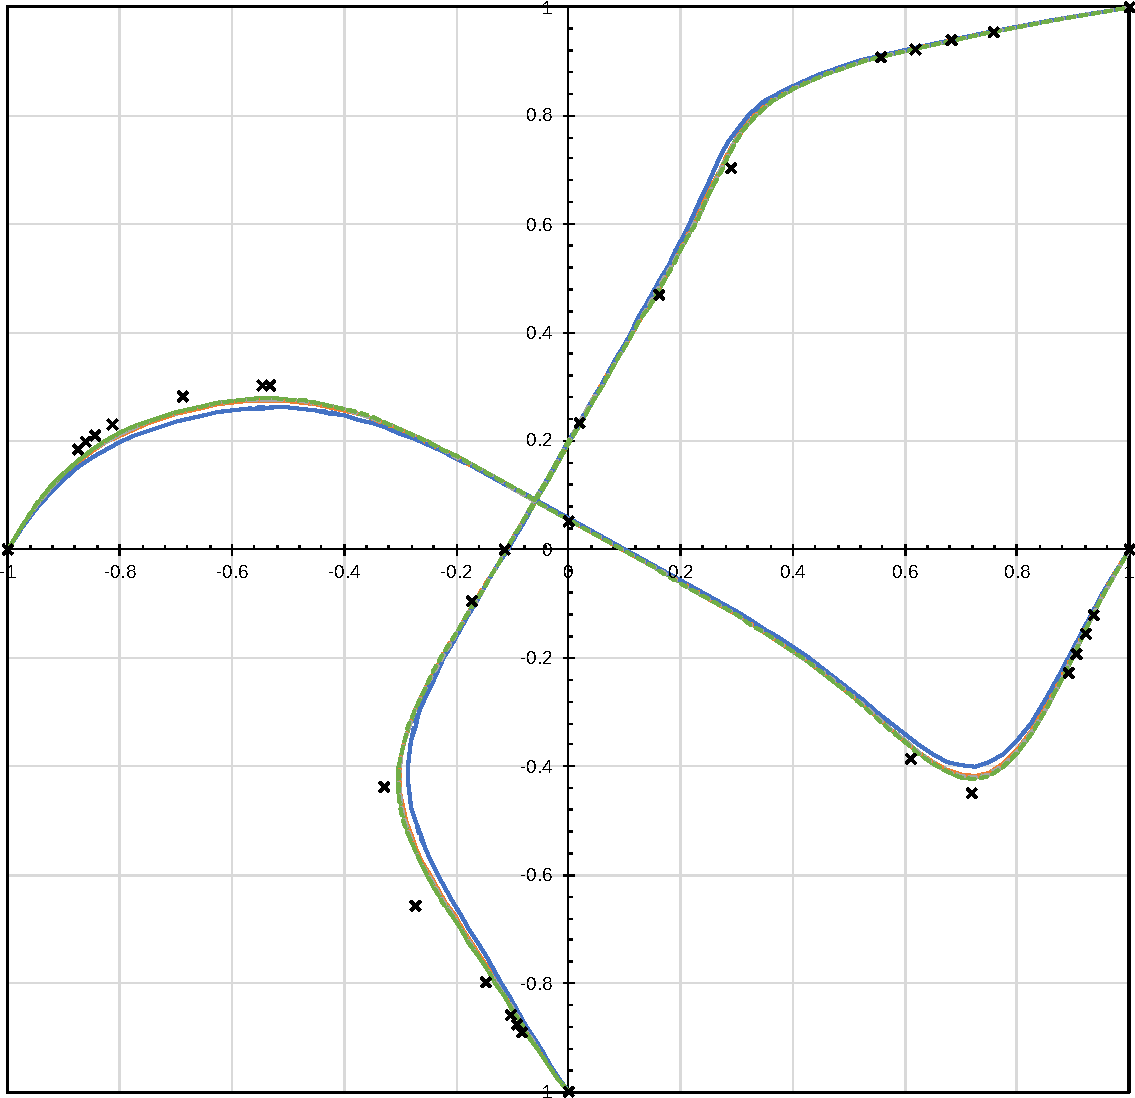
\includegraphics[width=\linewidth]{Figuras/Cavity/Re400.pdf}
        \caption{$\Rey=400$}
    \end{subfigure}
    \begin{subfigure}{0.4\textwidth}
        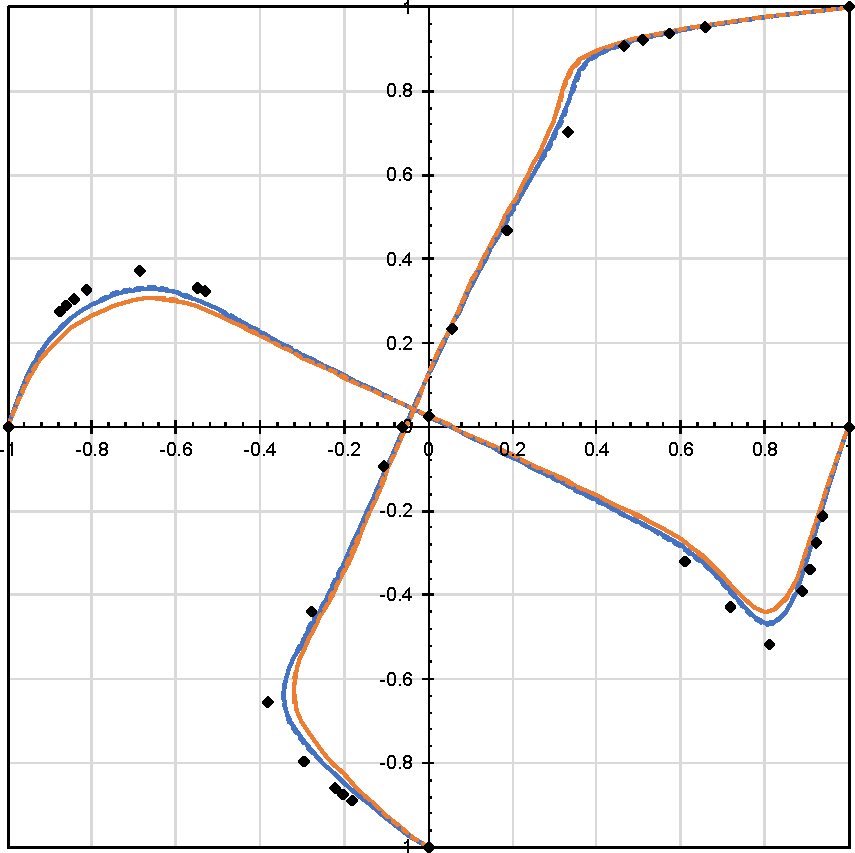
\includegraphics[width=\linewidth]{Figuras/Cavity/Re1000.pdf}
        \caption{$\Rey=1000$}
    \end{subfigure}
    \begin{subfigure}{0.4\textwidth}
        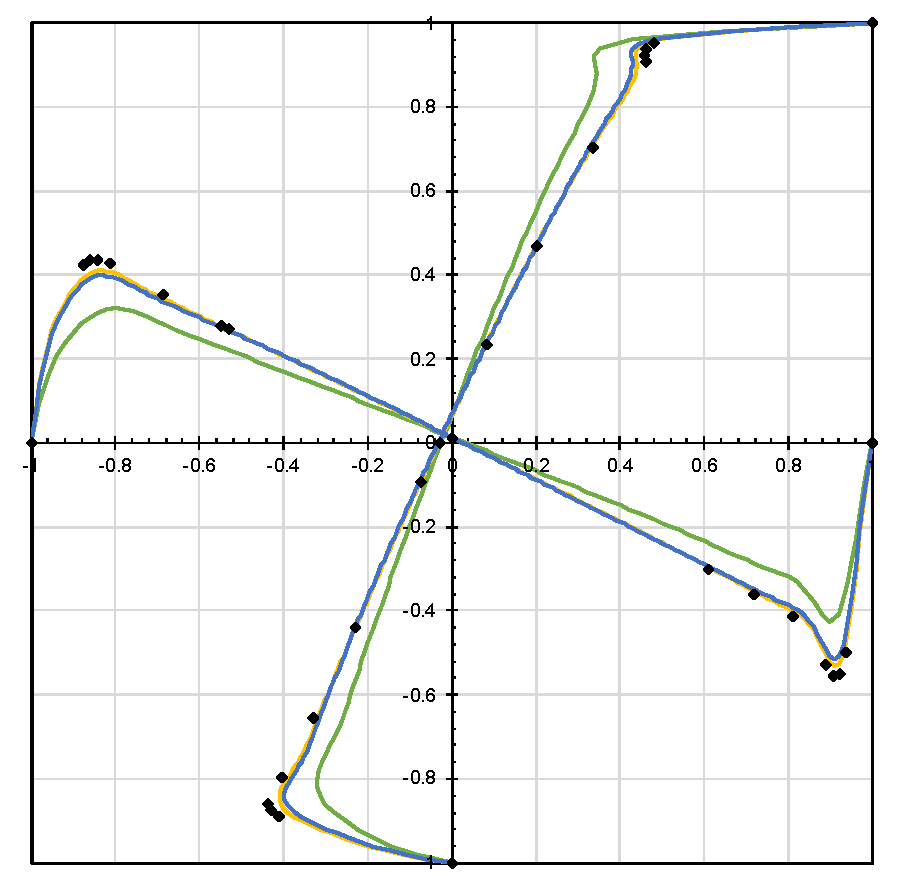
\includegraphics[width=\linewidth]{Figuras/Cavity/Re5000.pdf}
        \caption{$\Rey=5000$}
    \end{subfigure}
    \begin{subfigure}{0.4\textwidth}
        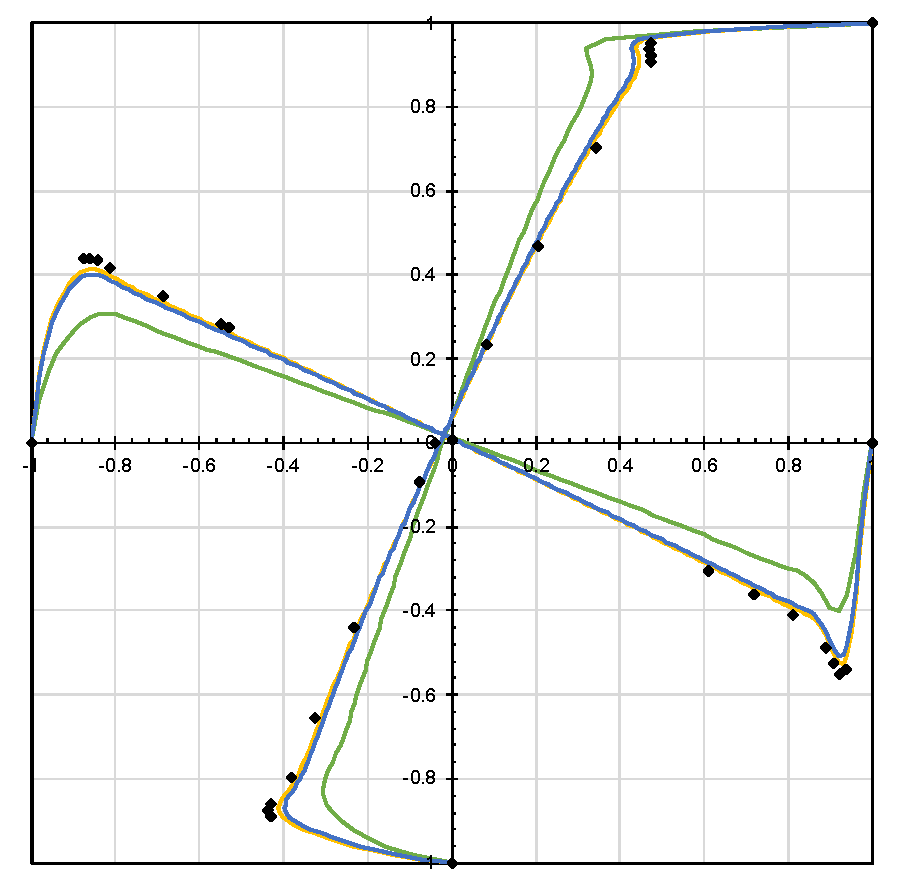
\includegraphics[width=\linewidth]{Figuras/Cavity/Re7500.pdf}
        \caption{$\Rey=7500$}
    \end{subfigure}
    \begin{subfigure}{0.4\textwidth}
        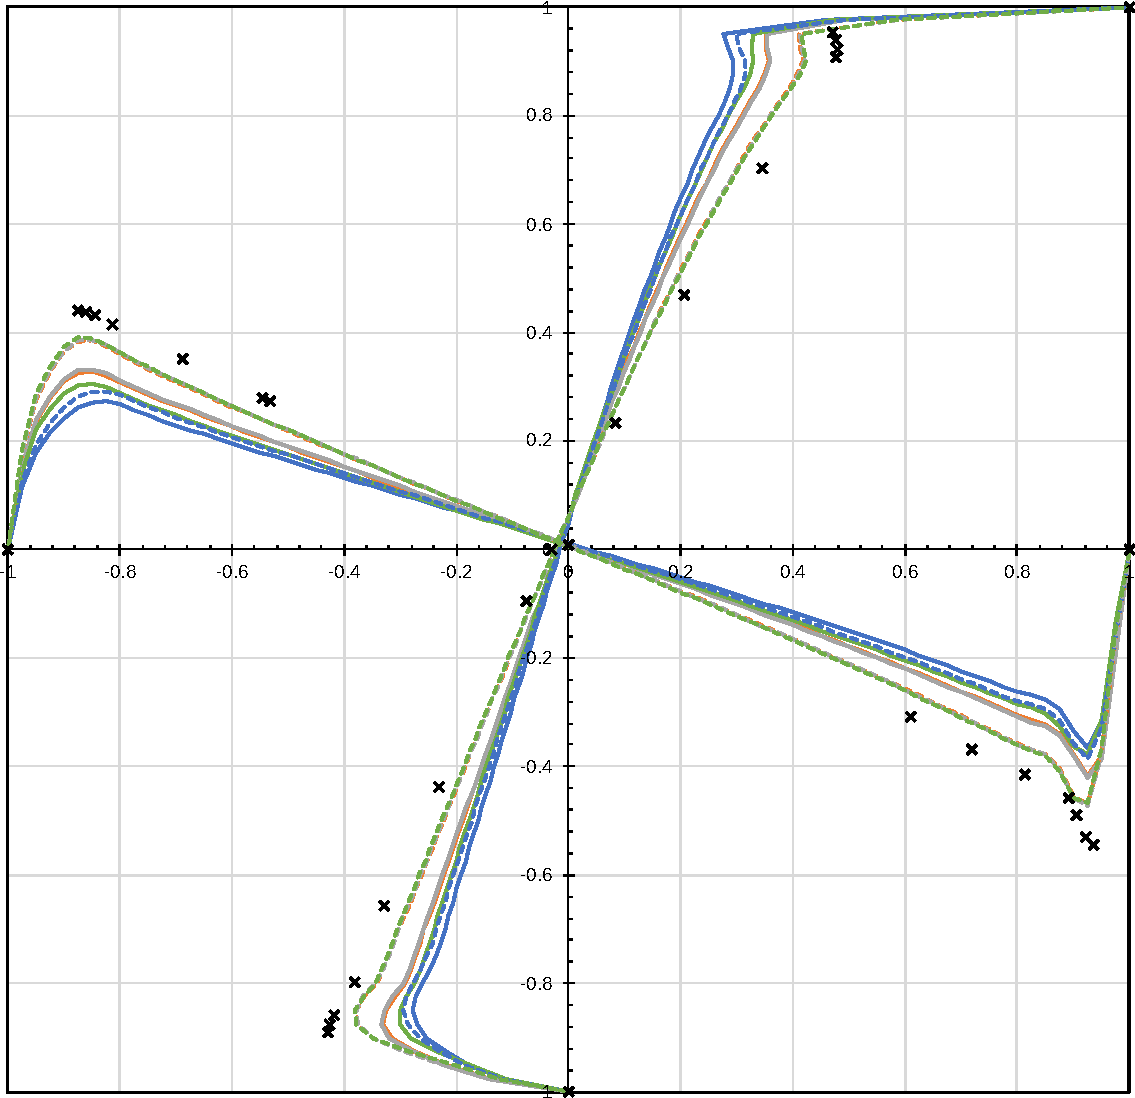
\includegraphics[width=\linewidth]{Figuras/Cavity/Re10000.pdf}
        \caption{$\Rey=10000$}
    \end{subfigure}
    \begin{subfigure}{\textwidth}
        \centering
        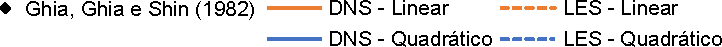
\includegraphics[width=.7\linewidth]{Figuras/Cavity/legenda.pdf}
    \end{subfigure}
    \\Fonte: Presente trabalho (\the\year).
    \label{fig:cavity-results}
\end{figure}

Pelo fato de se utilizar um método diferente em relação à referência, o qual utiliza o método \textit{multi-grid} com 257$\times$257 e 129$\times$129 pontos, percebe-se uma certa discrepância entre os resultados, especialmente à medida que o número de Reynolds aumenta. Nota-se ainda que a discretização com elementos P1P1, mesmo possuindo o mesmo número de graus de liberdade da discretização com elementos P2P2, apresenta resultados menos precisos. Isso se deve à representação mais pobre dos campos mecânicos pelos elementos P1P1.

Para todos os casos, à medida que o número de Reynolds aumenta, é possível notar que a aplicação do modelo LES melhorou a representação do campo de velocidade, o que deve-se à boa capacidade do modelo de capturar os efeitos turbulentos em escalas menores que os elementos da malha. Já o uso da formulação VMS, embora tenha sido muito eficiente para garantir a estabilização, não apresentou diferenças significativas em relação à formulação estabilizada SUPG/PSPG.

O emprego dos elementos P2P1 sem modelo de turbulência mostrou-se muito boa para representar o campo de velocidade, com resultados ligeiramente inferiores aos dos elementos P2P2 em formulação SUPG/PSPG observáveis apenas para os $Re=7.500$ e $Re=10.000$. É importante ainda notar que, embora o problema considerado atinja números de Reynolds elevados, os termos convectivos não atuam sobre fortes gradientes, de modo que foi possível obter solução estável com os elementos P2P1.

Com relação ao tempo de processamento, para as simulações apenas com estabilização SUPG/PSPG, observa-se um tempo médio de 0,2285 segundos por iteração na solução do problema não linear para a simulação com elementos P1P1, enquanto para a simulação com elementos P2P2 o tempo médio foi de 0,2032 segundos por iteração, o que resulta em um tempo 12,466\% maior para a simulação com elementos P1P1, ainda conduzindo a resultados menos precisos. Todavia, para a simulação com o modelo LES, o tempo médio de processamento foi de 0,2134 segundos por iteração em elementos P2P2, o que resulta em um tempo 5,028\% maior que o caso anterior, o que mostra que o modelo LES pode apresentar um certo impacto no tempo de processamento.

A Figura \ref{fig:cavity-results2} apresenta as distribuições do módulo da velocidade após o escoamento atingir seu estado estacionário, obtidas por meio da simulação com elementos P2P2 com VMS+LES.

\begin{figure}[h!]
    \centering
    \caption{Cavidade bidimensional - Campo de velocidade em regime estacionário.}
    \begin{subfigure}{0.32\textwidth}
        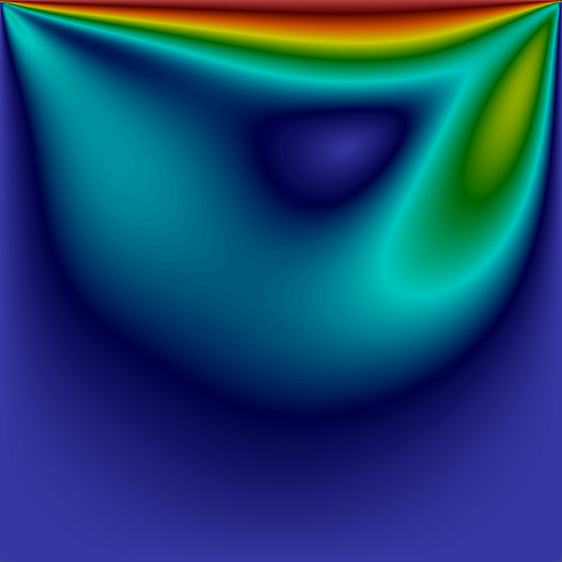
\includegraphics[width=\linewidth]{Figuras/Cavity/Re100.png}
        \caption{$\Rey=100$}
    \end{subfigure}
    \begin{subfigure}{0.32\textwidth}
        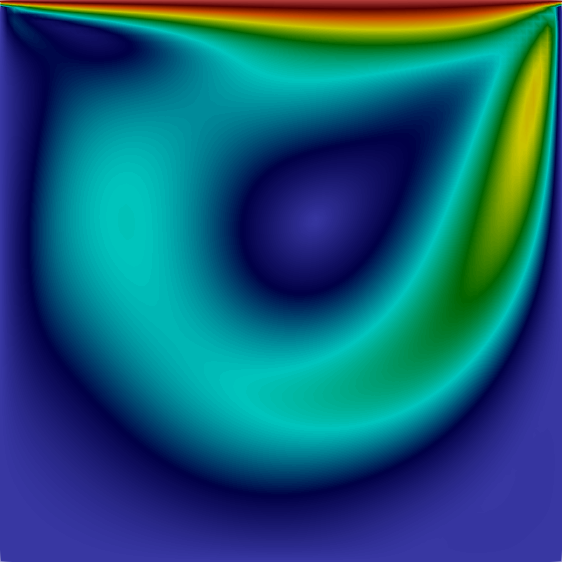
\includegraphics[width=\linewidth]{Figuras/Cavity/Re400.png}
        \caption{$\Rey=400$}
    \end{subfigure}
    \begin{subfigure}{0.32\textwidth}
        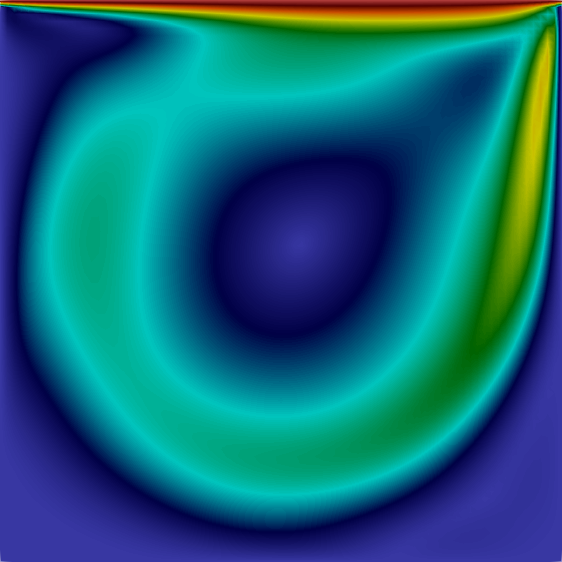
\includegraphics[width=\linewidth]{Figuras/Cavity/Re1000.png}
        \caption{$\Rey=1000$}
    \end{subfigure}
    \begin{subfigure}{0.32\textwidth}
        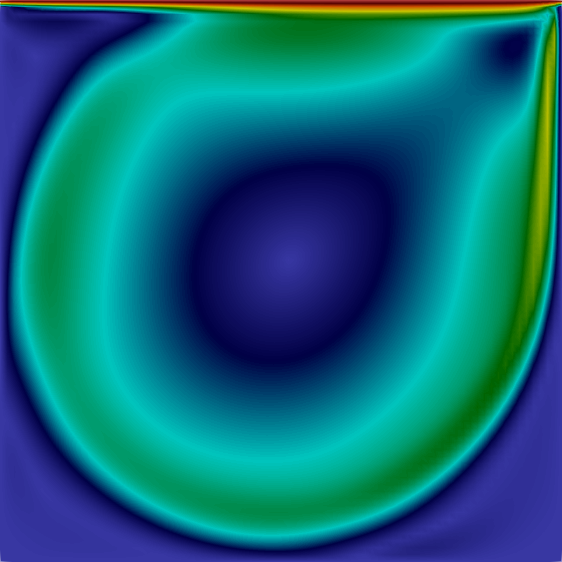
\includegraphics[width=\linewidth]{Figuras/Cavity/Re5000.png}
        \caption{$\Rey=5000$}
    \end{subfigure}
    \begin{subfigure}{0.32\textwidth}
        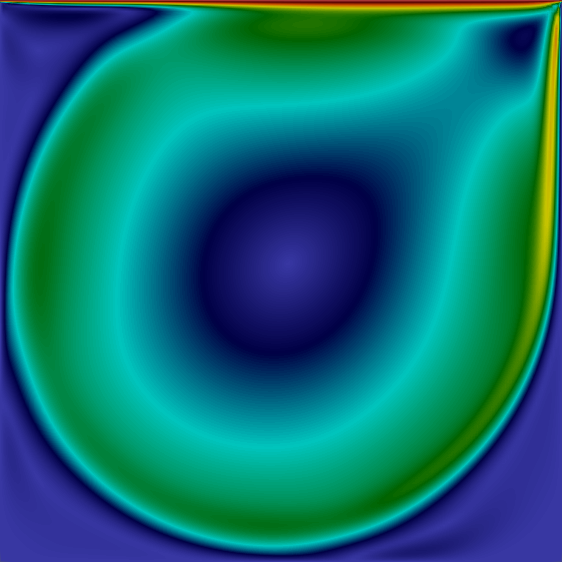
\includegraphics[width=\linewidth]{Figuras/Cavity/Re7500.png}
        \caption{$\Rey=7500$}
    \end{subfigure}
    \begin{subfigure}{0.32\textwidth}
        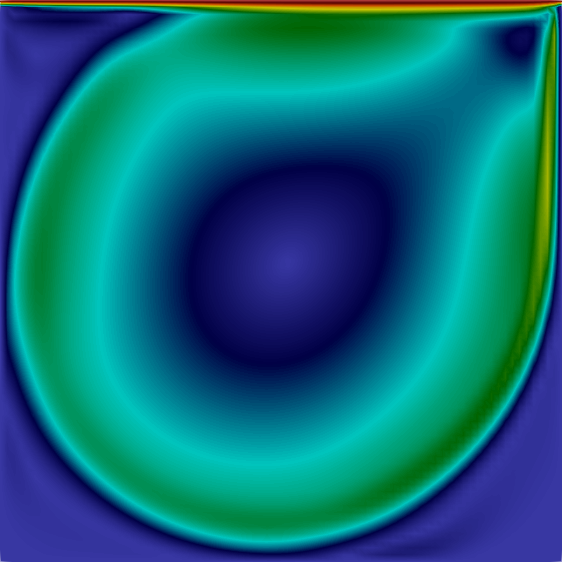
\includegraphics[width=\linewidth]{Figuras/Cavity/Re10000.png}
        \caption{$\Rey=10000$}
    \end{subfigure}
    \begin{subfigure}{0.4\textwidth}
        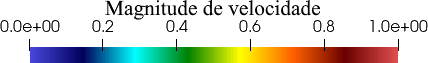
\includegraphics[width=\linewidth]{Figuras/Cavity/legenda.png}
    \end{subfigure}
    \\Fonte: Presente trabalho (\the\year).
    \label{fig:cavity-results2}
\end{figure}


Como todas as simulações anteriores se mostram estáveis e consistentes para atingir a solução estacionária, são propostas as discretizações menos refinadas conforme a tabela \ref{tab:cavity-mesh2}, ilustradas na figura \ref{fig:cavity-mesh2}, para simulações do problema com $\Rey=10.000$ empregando-se elementos P2P2 com estabilização SUPG/PSPG e elementos P2P1 estabilizados com SUPG, bem como a combinação desses casos com o LES. Descartaram-se as outras combinações por terem apresentado resultados inferiores ou sem diferenças significativas em relação aos casos considerados agora.

\begin{table}[h!]
    \centering
    \caption{Cavidade bidimensional - Características das malhas utilizadas para a análise de dependência.}
    \begin{tabular}{lcccccc}
        \hline
        Malha               & Elemento & Subdivisões & Elementos & $n_u$ & $n_p$ & DOF  \\\hline
        \multirow{2}{*}{m1} & P2P2     & 20          & 800       & 1681  & 1681  & 5043 \\
                            & P2P1     & 20          & 800       & 1681  & 441   & 3803 \\\hline
        m2                  & P2P2     & 8           & 128       & 289   & 289   & 867  \\\hline
    \end{tabular}
    \\Fonte: Presente trabalho (\the\year).
    \label{tab:cavity-mesh2}
\end{table}

\begin{figure}[h!]
    \centering
    \caption{Cavidade bidimensional - Malhas utilizadas para a análise de convergência.}
    \begin{subfigure}{0.49\textwidth}
        \centering
        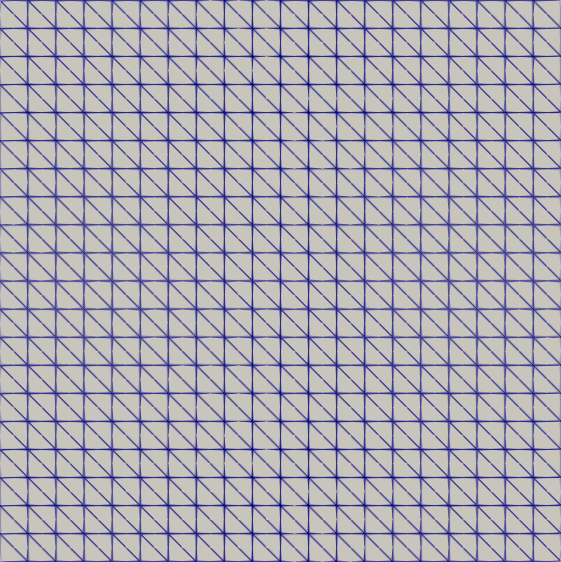
\includegraphics[width=0.8\linewidth]{Figuras/Cavity/m2.png}
        \caption{Malha m1.}
    \end{subfigure}
    \begin{subfigure}{0.49\textwidth}
        \centering
        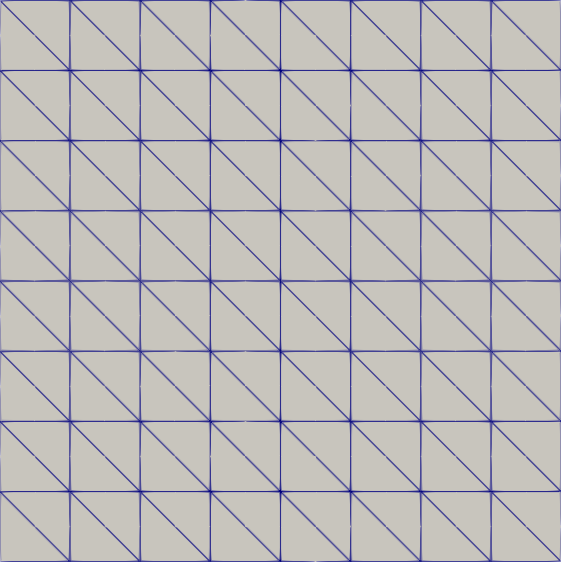
\includegraphics[width=0.8\linewidth]{Figuras/Cavity/m3.png}
        \caption{Malha m2.}
    \end{subfigure}
    \\Fonte: Presente trabalho (\the\year).
    \label{fig:cavity-mesh2}
\end{figure}

Para essas simulações, o elemento P2P1 não apresentou convergência para a malha m1, mesmo com o emprego do modelo LES, o que pode ser explicado pela baixa ordem de aproximação do campo de pressão, que conduz à resultados mais imprecisos conforme a malha se torna mais grosseira. Já para a malha m2 se observou a não convergência também para o caso de elementos P2P2 com estabilização SUPG/PSPG, enquanto a sua combinação com o LES se manteve estável durante toda a análise. A Figura \ref{fig:cavity-results3} apresenta a distribuição de velocidade sobre as linhas médias da cavidade para as simulações que apresentaram convergência.

\begin{figure}[h!]
    \centering
    \caption{Cavidade bidimensional - Valores do campo de velocidade sobre as linhas médias para as malhas m1 e m2.}
    \begin{subfigure}{0.49\textwidth}
        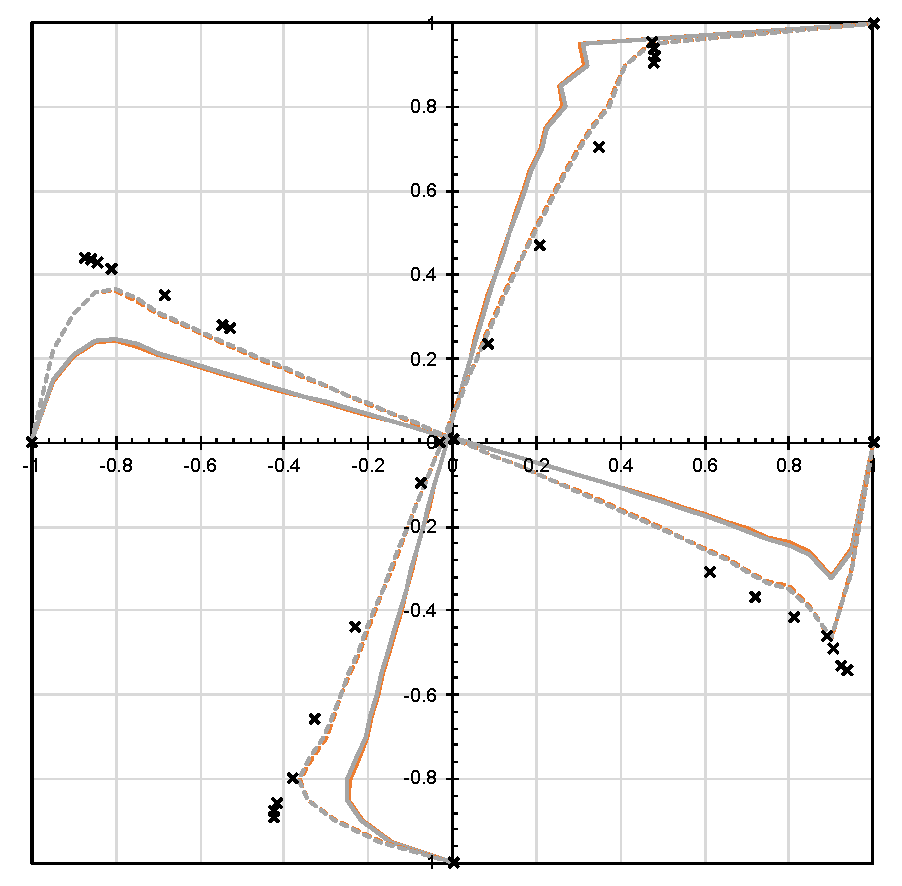
\includegraphics[width=\linewidth]{Figuras/Cavity/res-m1.pdf}
        \caption{Malha m1.}
    \end{subfigure}
    \begin{subfigure}{0.49\textwidth}
        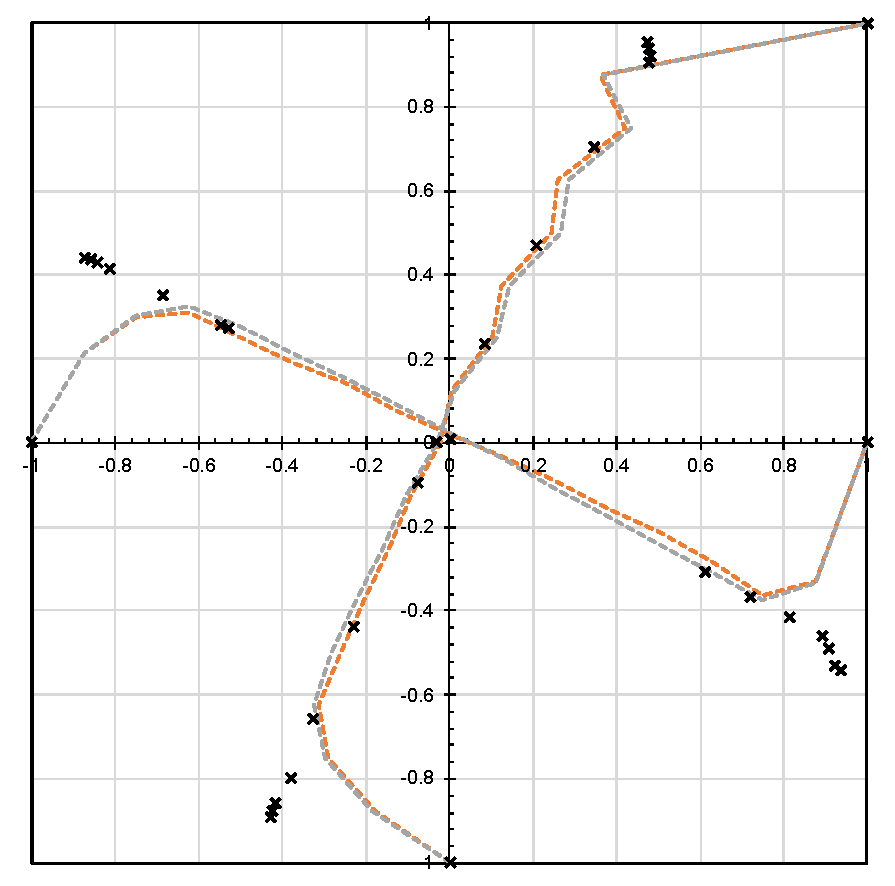
\includegraphics[width=\linewidth]{Figuras/Cavity/res-m2.pdf}
        \caption{Malha m2.}
    \end{subfigure}
    \begin{subfigure}{0.4\textwidth}
        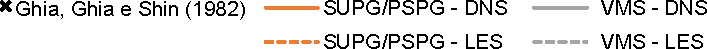
\includegraphics[width=\linewidth]{Figuras/Cavity/legenda-m1m2.pdf}
    \end{subfigure}
    \\Fonte: Presente trabalho (\the\year).
    \label{fig:cavity-results3}
\end{figure}

Com base nesses resultados, constata-se que a aplicação do modelo LES é capaz de garantir maior precisão e estabilidade mesmo para discretizações mais grosseiras. Também se observa que a consideração dos demais termos estabilizadores da formulação VMS promoveu uma melhora pequena em relação à simulação estabilizada por SUPG/PSPG apenas nos casos de número de Reynolds mais elevados.

Por fim, estuda-se o mesmo problema considerando um discretização tridimensional definida pelo domínio cúbico $\Omega=[-1,1]^3$, onde as condições impostas nas faces frontal e traseira são de paredes lisas. A malha utilizada nesse caso é estruturada apenas nas faces do cubo, como ilustrada na figura \ref{fig:cavity-mesh3}, sendo composta por 8154 elementos P2P2, com 12557 nós e 50228 graus de liberdade.

\begin{figure}[h!]
    \centering
    \caption{Cavidade tridimensional - Malha utilizada.}
    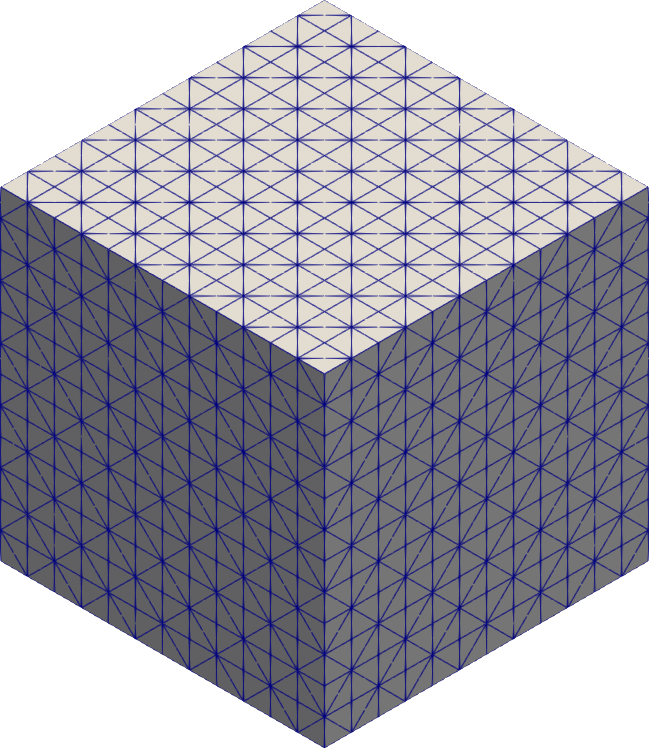
\includegraphics[width=0.4\linewidth]{Figuras/cavity3D/malha.png}
    \\Fonte: Presente trabalho (\the\year).
    \label{fig:cavity-mesh3}
\end{figure}

O problema foi estudado para as estabilizações SUPG/PSPG, com e sem a aplicação de LES, para $\Rey=100$, $400$ e $1000$. A Figura \ref{fig:cavity-results4} apresenta a distribuição de velocidade sobre as linhas médias verticais e horizontais da cavidade.

\begin{figure}[h!]
    \centering
    \caption{Cavidade tridimensional - Valores do campo de velocidade sobre as linhas médias.}
    \begin{subfigure}{0.49\textwidth}
        \centering
        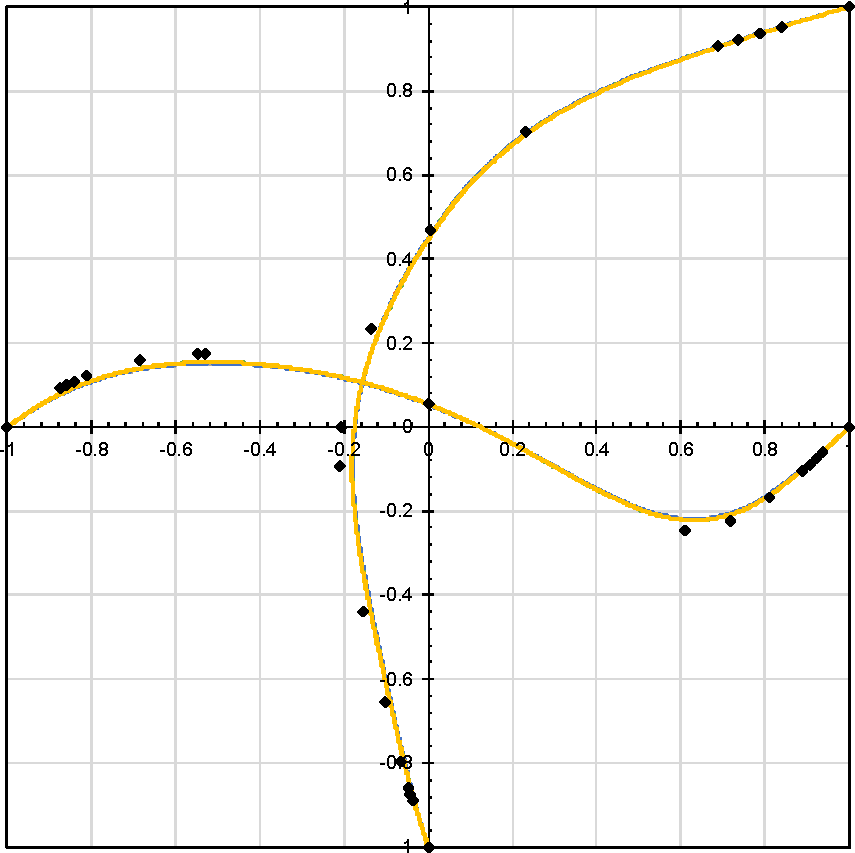
\includegraphics[width=\linewidth]{Figuras/cavity3D/Re100.pdf}
        \caption{$\Rey=100$}
    \end{subfigure}
    \begin{subfigure}{0.49\textwidth}
        \centering
        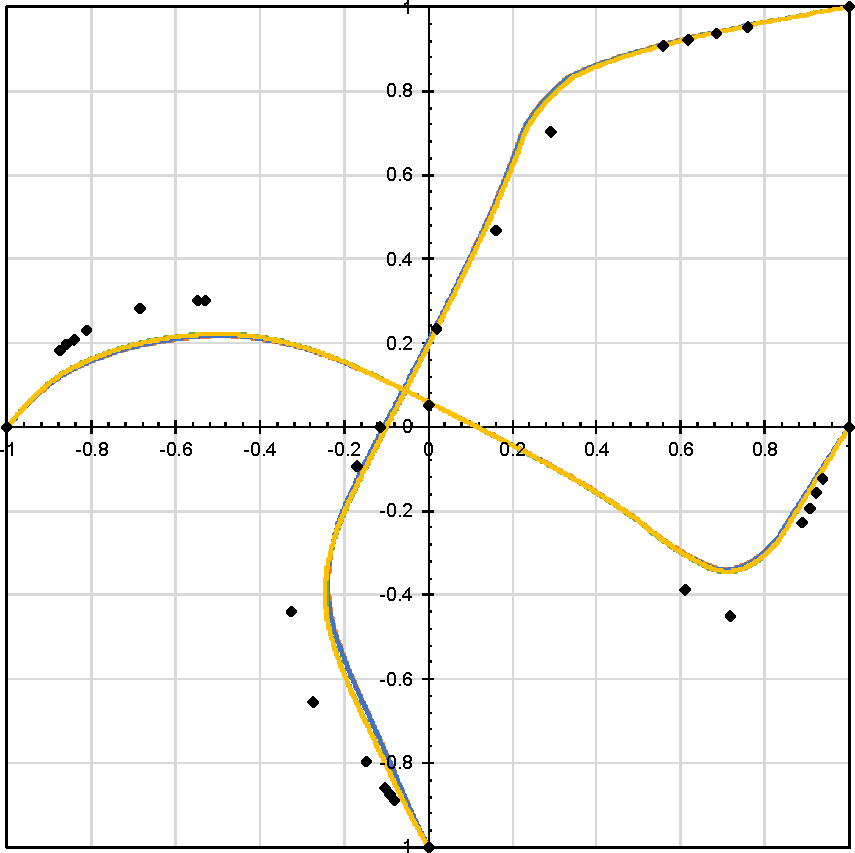
\includegraphics[width=\linewidth]{Figuras/cavity3D/Re400.pdf}
        \caption{$\Rey=400$}
    \end{subfigure}
    \begin{subfigure}{0.49\textwidth}
        \centering
        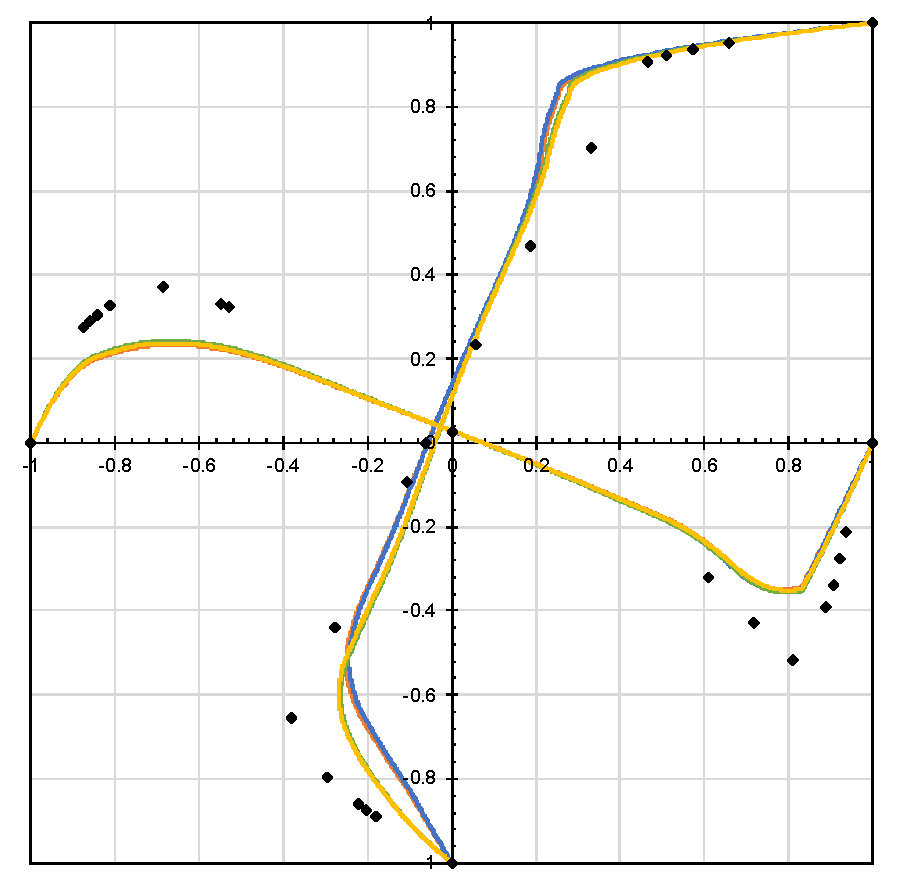
\includegraphics[width=\linewidth]{Figuras/cavity3D/Re1000.pdf}
        \caption{$\Rey=1000$}
    \end{subfigure}
    \begin{subfigure}{\textwidth}
        \centering
        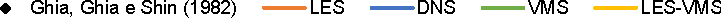
\includegraphics[width=0.5\linewidth]{Figuras/cavity3D/legenda.pdf}
    \end{subfigure}
    \\Fonte: Presente trabalho (\the\year).
    \label{fig:cavity-results4}
\end{figure}

Pode-se perceber, então, que para números de Reynolds baixos o resultado não difere muito entre as diferentes simulações. No entanto, à medida que o número de Reynolds aumenta, a aplicação dos demais termos estabilizadores da formulação VMS melhorou a solução obtida em relação à simulação estabilizada por SUPG/PSPG. Já com relação à aplicação do LES, verifica-se que houve uma pequena melhora nos resultados, no entanto o $\Rey$ ainda foi pequeno o suficiente para que sua aplicação não fosse tão significativa.

Em seguida realizou-se uma simulação com uma malha ainda mais grosseira, com 2695 elementos P2P2 contendo 4360 nós e 17440 graus de liberdade para $\Rey=10000$, utilizando estabilização SUPG/PSPG, com e sem aplicação de LES, e VMS. A Figura \ref{fig:cavity-results5} apresenta o campo de velocidade obtido na face de simetria do problema para as diferentes simulações no instante $t=450$.

\begin{figure}[h!]
    \centering
    \caption{Cavidade tridimensional - Campo de velocidade na face de simetria.}
    \begin{subfigure}{0.32\textwidth}
        \centering
        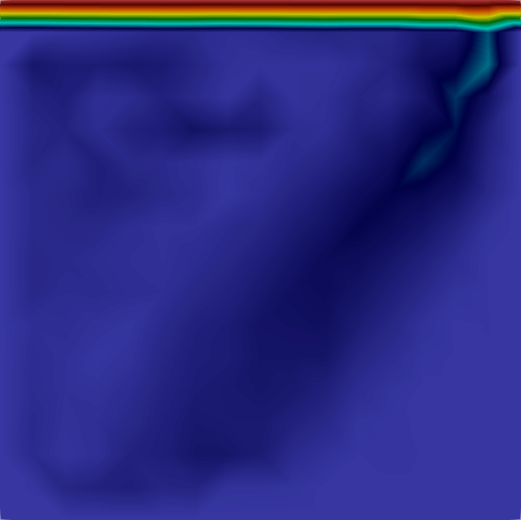
\includegraphics[width=\linewidth]{Figuras/cavity3D/DNS.png}
        \caption{SUPG/PSPG}
    \end{subfigure}
    \begin{subfigure}{0.32\textwidth}
        \centering
        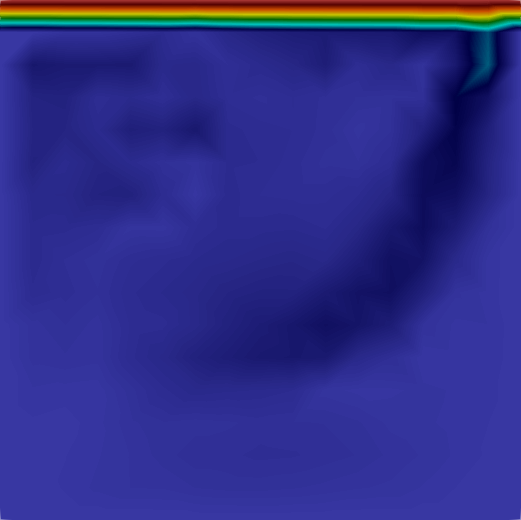
\includegraphics[width=\linewidth]{Figuras/cavity3D/VMS.png}
        \caption{VMS}
    \end{subfigure}
    \begin{subfigure}{0.32\textwidth}
        \centering
        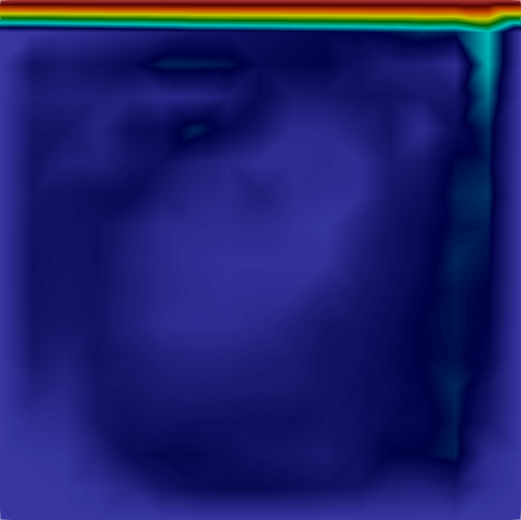
\includegraphics[width=\linewidth]{Figuras/cavity3D/LES.png}
        \caption{LES}
    \end{subfigure}
    \\Fonte: Presente trabalho (\the\year).
    \label{fig:cavity-results5}
\end{figure}

Analisando qualitativamente os resultados, observa-se que a aplicação do LES, mesmo para uma malha tão grosseira, foi capaz de melhorar a representação do campo de velocidade, enquanto a simulação sem aplicação do modelo de turbulência apresentou um resultado distante do esperado.

\begin{comment}
%==================================================================================================
\subsection{\textit{Taylor-Green Vortex} tridimensional}
%==================================================================================================

Para verificação dos modelos implementados em simulações tridimensionais é possível simular o problema de \textit{Taylor-Green Vortex} (TGV), o qual possui solução analítica, dada por \cite{shapiro1993use}:

\begin{subequations}
    \begin{equation}
        \begin{split}
            &\BB{u}_a(\BB{x},t)=\\
            &-\frac{Ae^{-\nu\lambda^2t}}{k^2+l^2}\begin{bmatrix}
                \lambda l\cos{(kx_1)}\sin{(lx_2)}\sin{(mx_3)}+mk\sin{(kx_1)}\cos{(lx_2)}\cos{(mx_3)} \\
                \lambda k\sin{(kx_1)}\cos{(lx_2)}\sin{(mx_3)}-ml\cos{(kx_1)}\sin{(lx_2)}\cos{(mx_3)} \\
                -(k^2+l^2)\cos{(kx_1)}\cos{(lx_2)}\sin{(mx_3)}
            \end{bmatrix}\text{,}
        \end{split}
    \end{equation}
    \begin{equation}
        p_a=p_s-\rho\frac{u_1^2+u_2+u_3^2}{2}\text{.}
    \end{equation}
\end{subequations}

\noindent em que $k$, $l$ e $m$ são constantes arbitrárias, $\lambda^2=k^2+l^2+m^2$, $A$ é a amplitude da componente $u_3$ e $p_s$ é a pressão do ponto de estagnação.

Para o problema numérico foi considerado um cubo ($\Omega=[-1,1]^3$) simulado nos modelos VMS de aproximação linear e quadrática e o LES utilizando elementos Taylor-Hood P2P1. A malha utilizada na discretização conta com 5802 elementos finitos (conforme ilustrado na Figura \ref{fig:TGV-mesh}), sendo 5580 graus de liberdade para VMS linear, 37600 pra VMS quadrático e 29595 para LES.

\begin{figure}[h!]
    \centering
    \caption{Malha utilizada para a simulação de TGV.}
    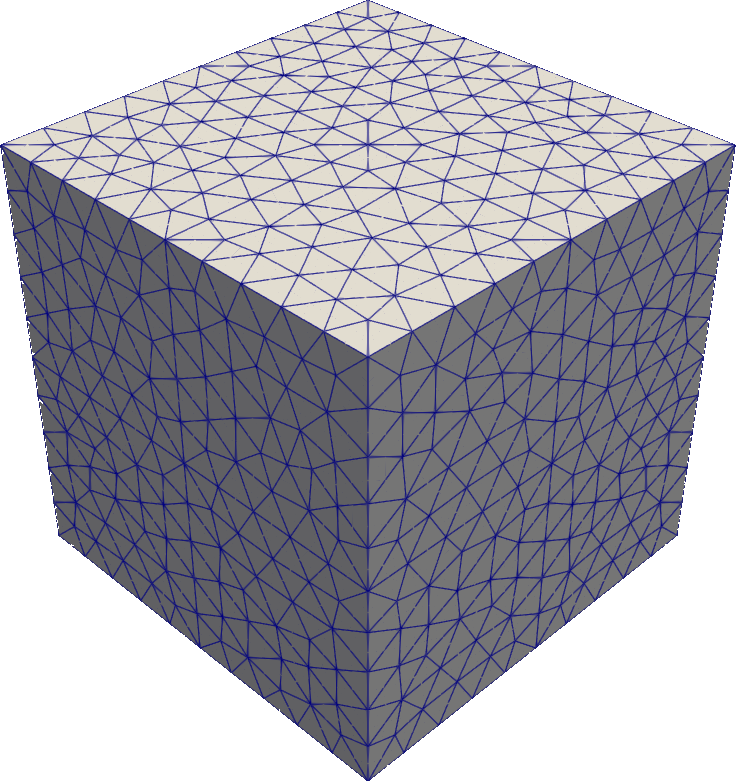
\includegraphics[width=0.4\linewidth]{Figuras/taylor-green/mesh.png}
    \\Fonte: Presente trabalho (\the\year).
    \label{fig:TGV-mesh}
\end{figure}

Como condição inicial impôs-se acelerações, velocidade e pressões iguais à solução analítica com $t=0$ e como condições de contorno aplicou-se velocidades iguais à analítica em toda a fronteira e $p=0$ no centro do domínio. Os valores dos parâmetros foram $k=l=m=\pi$ e $A=\nu=\rho=1$, sendo o período analisado de $t\in[0,0.2]$ com um passo de tempo de $\Delta t=0.001$.

Sendo assim, a Figura \ref{fig:TGV-results} apresenta os valores do campo de velocidades nas linhas $x_2=x_3=0$ ($l1$), $x_1=x_3=0$ ($l2$) e $x_1=x_2=0$ ($l3$) para os instantes $t=0$, $t=0.05$ e $t=0.2$ para todos os modelos considerados.

\begin{figure}[h!]
    \centering
    \caption{Velocidades obtidas na simulação de TGV em:}
    \begin{subfigure}{0.42\textwidth}
        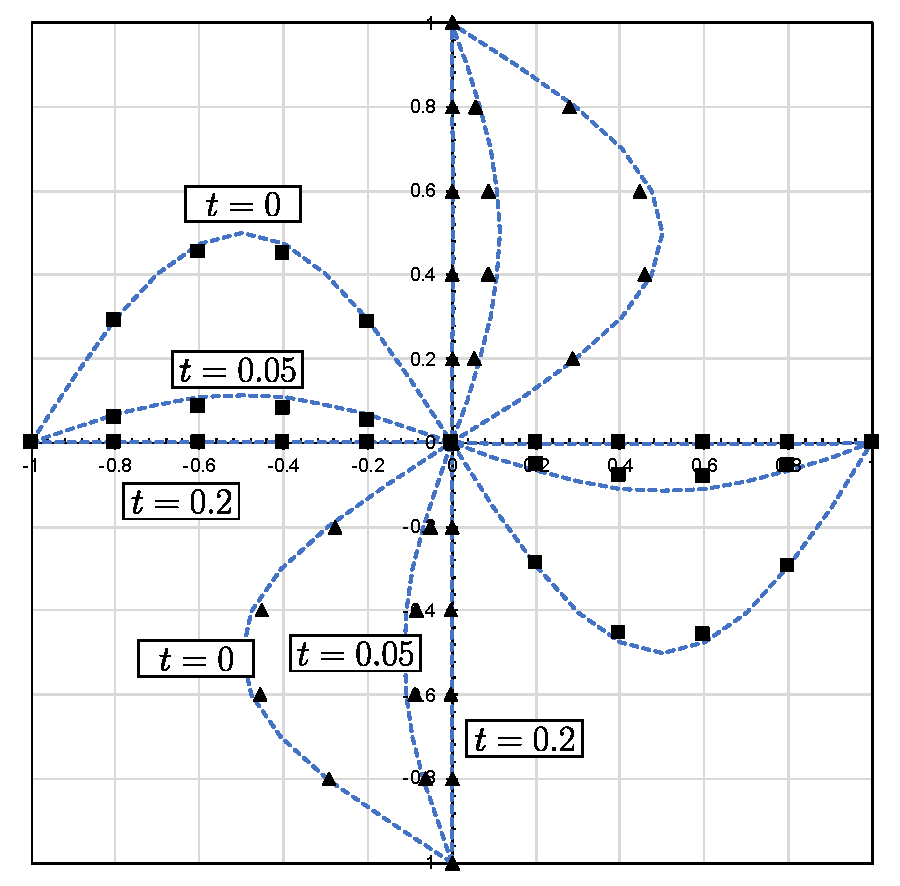
\includegraphics[width=\linewidth]{Figuras/taylor-green/VMS-Lin.pdf}
        \caption{$l1$ e $l2$ para VMS linear.}
    \end{subfigure}
    \begin{subfigure}{0.42\textwidth}
        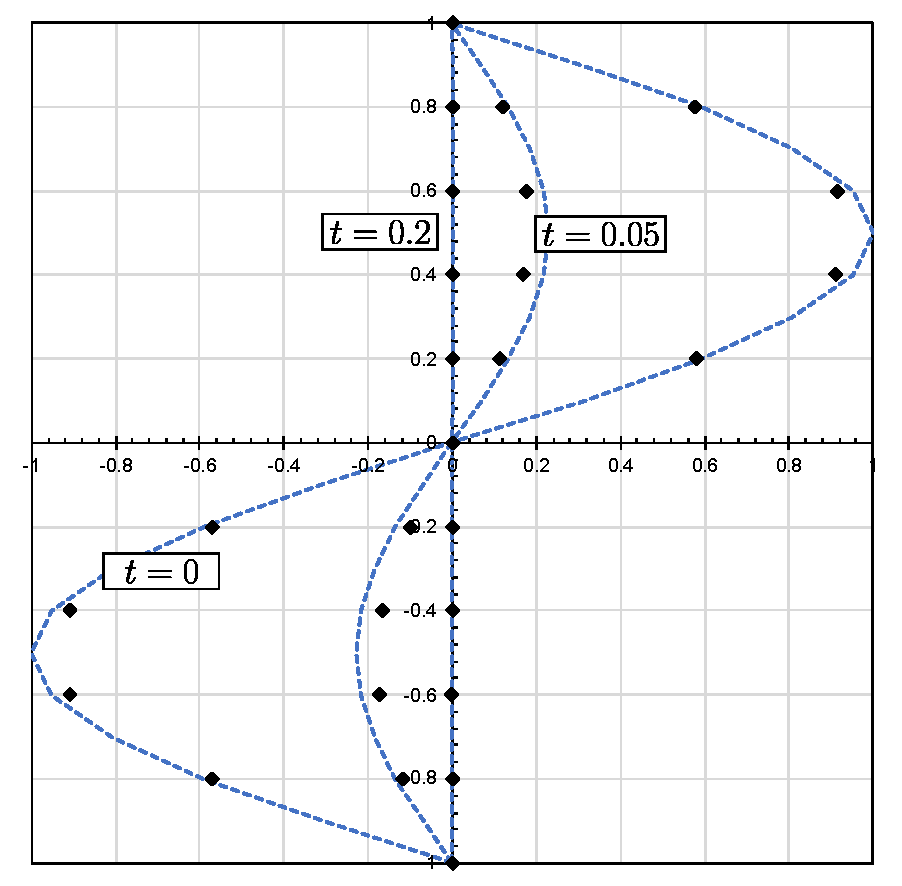
\includegraphics[width=\linewidth]{Figuras/taylor-green/VMS-Lin-uz.pdf}
        \caption{$l3$ para VMS linear.}
    \end{subfigure}
    \begin{subfigure}{0.42\textwidth}
        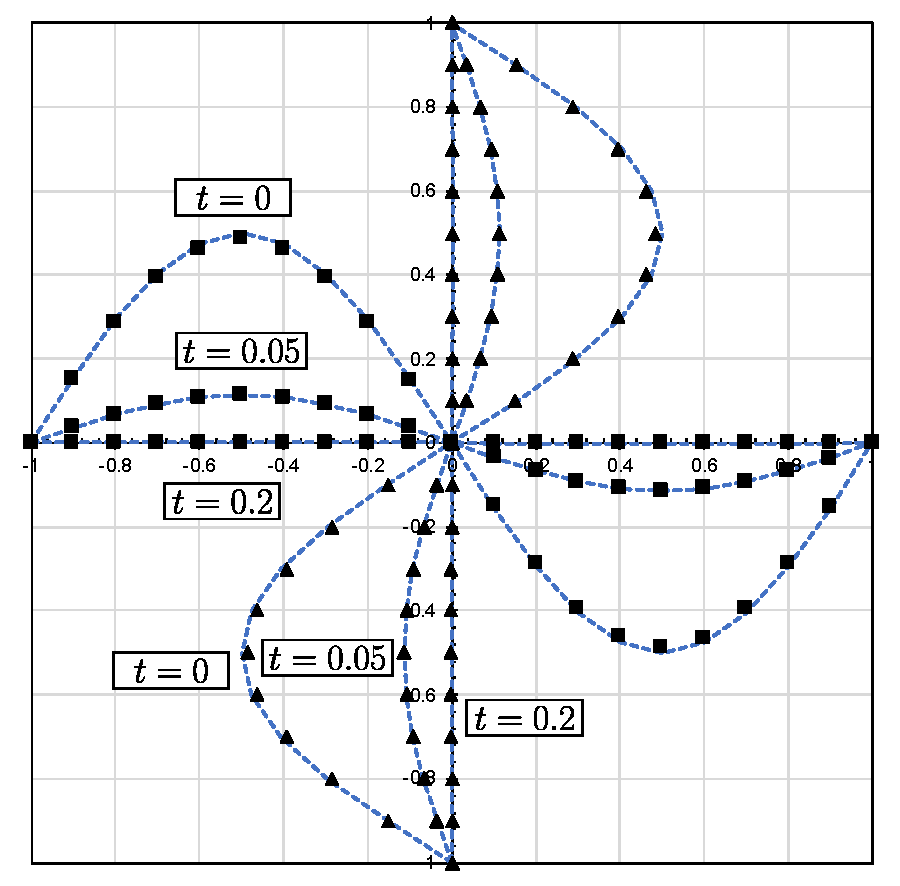
\includegraphics[width=\linewidth]{Figuras/taylor-green/VMS-Qua.pdf}
        \caption{$l1$ e $l2$ para VMS quadrático.}
    \end{subfigure}
    \begin{subfigure}{0.42\textwidth}
        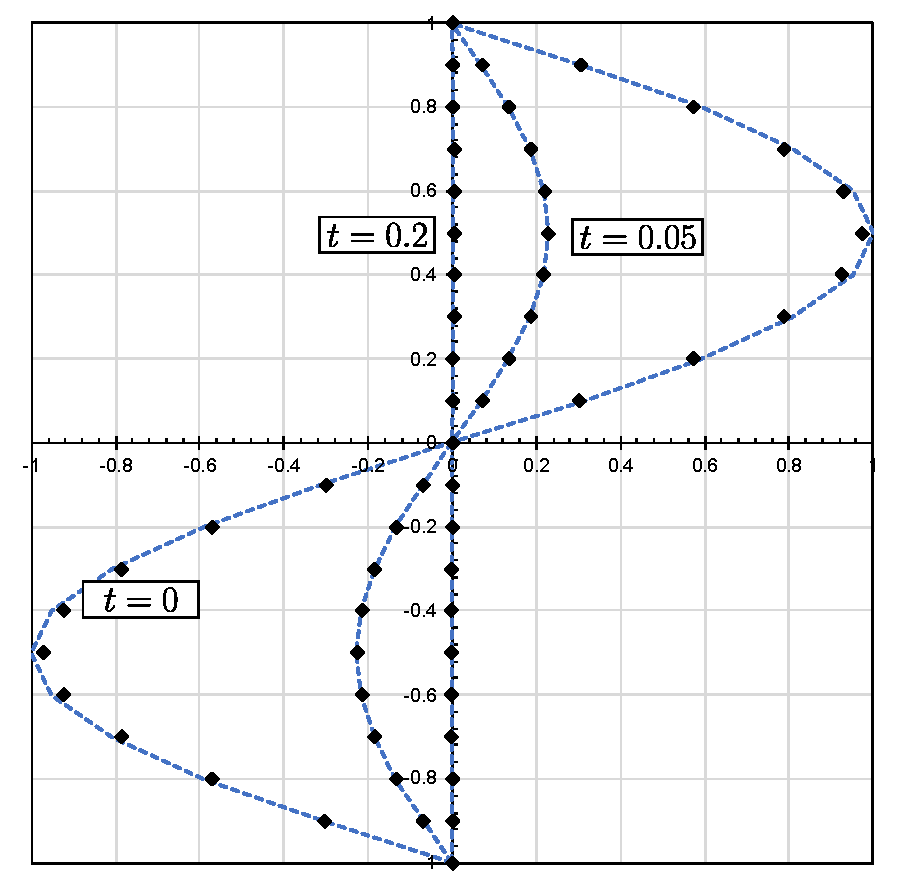
\includegraphics[width=\linewidth]{Figuras/taylor-green/VMS-Qua-uz.pdf}
        \caption{$l3$ para VMS quadrático.}
    \end{subfigure}
    \begin{subfigure}{0.42\textwidth}
        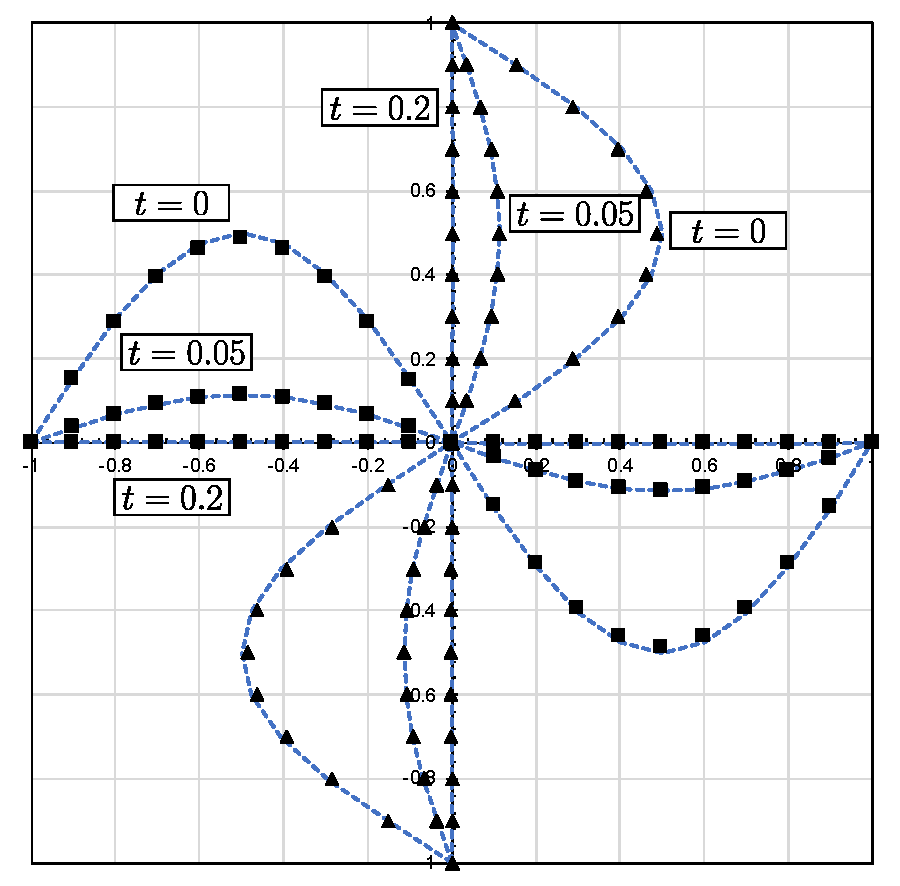
\includegraphics[width=\linewidth]{Figuras/taylor-green/LES.pdf}
        \caption{$l1$ e $l2$ para LES.}
    \end{subfigure}
    \begin{subfigure}{0.42\textwidth}
        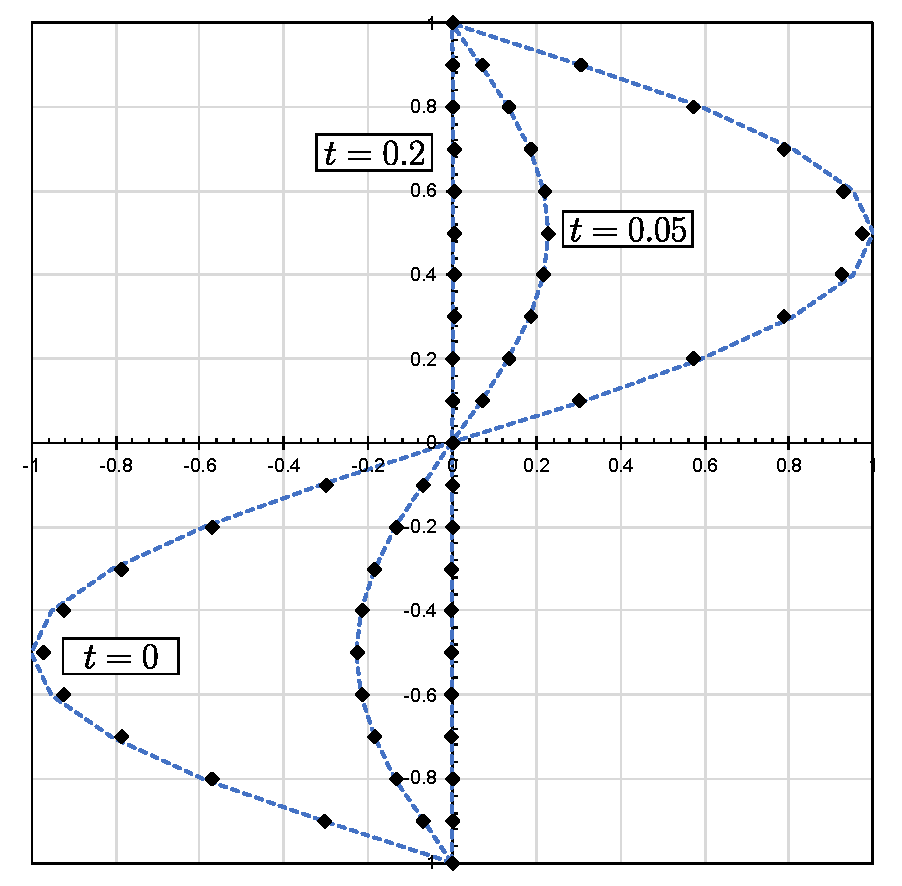
\includegraphics[width=\linewidth]{Figuras/taylor-green/LES-uz.pdf}
        \caption{$l3$ para LES.}
    \end{subfigure}
    \begin{subfigure}{0.42\textwidth}
        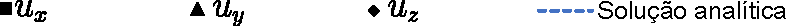
\includegraphics[width=\linewidth]{Figuras/taylor-green/legenda.pdf}
    \end{subfigure}
    \\Fonte: Presente trabalho (\the\year).
    \label{fig:TGV-results}
\end{figure}

Para comparação com a solução analítica, tomou-se a medida do erro em $L^2$, expresso por \cite{dumon2011proper}:

\begin{equation}
    \norm{\BB{e}}=\norm{\BB{u}-\BB{u}_a}_{L^\infty(L^2(\Omega))}=\max_{0<t\leq T}{\left[\int_\Omega{\norm{\BB{u}-\BB{u}_a}^2d\Omega}\right]}\text{,}
\end{equation}

\noindent o qual é representado ao longo do tempo de acordo com a Figura \ref{fig:TGV-L2}:

\begin{figure}[h!]
    \centering
    \caption{Medidas de $L^2$ ao longo do tempo.}
    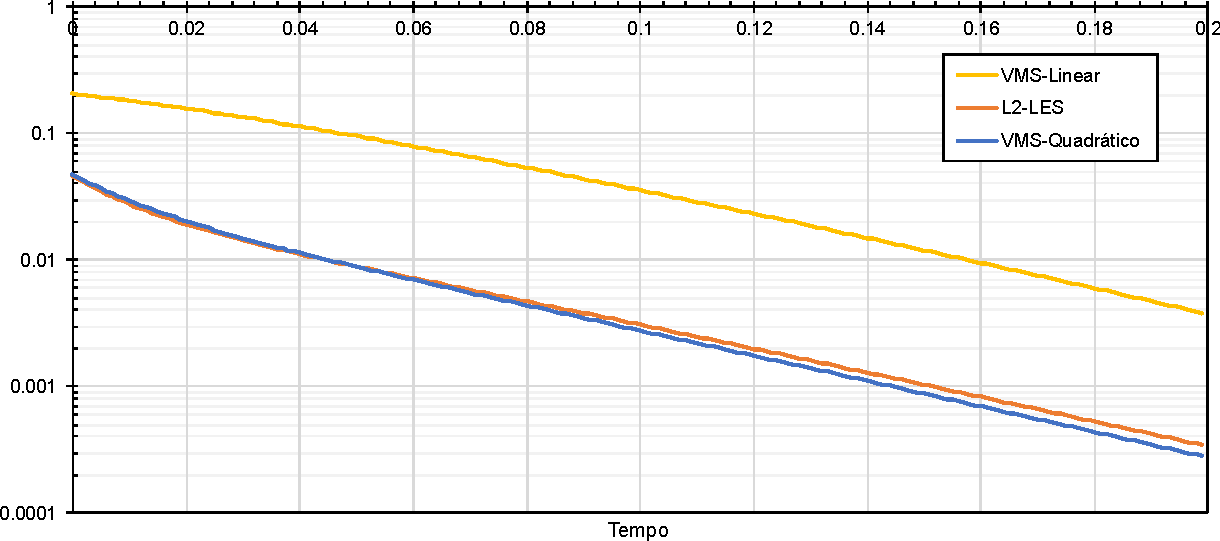
\includegraphics[width=\linewidth]{Figuras/taylor-green/L2.pdf}
    \\Fonte: Presente trabalho (\the\year).
    \label{fig:TGV-L2}
\end{figure}

Assim, observa-se que para o problema estudado, tanto as simulações VMS de aproximação quadrática quanto LES com elemento P2P1 apresentaram boa concordância com o resultado analítico, sendo que ambos apresentaram erros muito próximos entre si, enquanto o VMS de aproximação linear já apresentou um erro maior. Analisando o instante $t=0.1$ obteve-se um erro $L^2$ de $3,55\times 10^{-2}$, $2,77\times 10^{-3}$ e $3,07\times 10^{-3}$ para as simulações VMS linear, quadrático e LES, respectivamente. Ao verificar a ordem da medida do erro, observa-se que estes valores se encontram próximos ao obtido por \citeonline{zapata2023parallel}. Realizando uma regressão exponencial do tipo \[\norm{\BB{e}}=a\cdot10^{mt}\] para $t\geq 0,1$, encontra-se $m=-9,80$, $m=-10,01$ e $m=-9,60$ para os respectivos modelos.
\end{comment}

%==================================================================================================
\subsection{Escoamento em degrau invertido} \label{ex:backwardFacingStep}
%==================================================================================================

O problema de escoamento em degrau invertido é um problema clássico de escoamento em dutos, sendo bastante utilizado como \textit{benchmark} \cite{armaly1983experimental,chiang1999numerical}. O problema consiste em um escoamento advindo de um duto, cuja seção sofre um alargamento abrupto, conforme ilustrado na Figura \ref{fig:step}. Tal problema tem sua origem nos estudos experimentais de \citeonline{armaly1983experimental} e posteriormente estudado numericamente em problemas tridimensionais por \citeonline{chiang1999numerical}.

\begin{figure}[h!]
    \centering
    \caption{Escoamento em degrau invertido - Desenho esquemático.}
    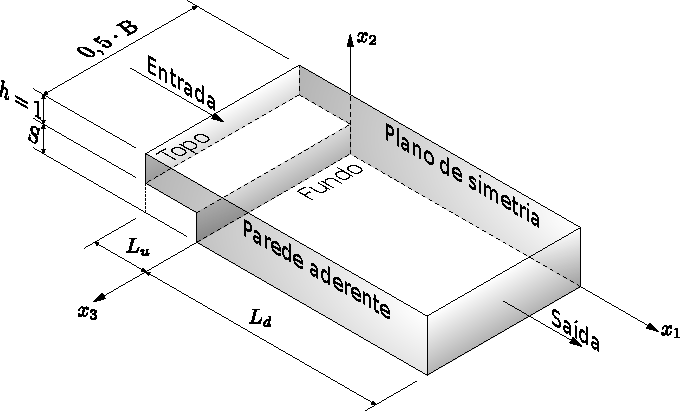
\includegraphics[width=.7\linewidth]{Figuras/backwardFacingStep/backwardFacingStep.pdf}
    \\Fonte: Presente trabalho (\the\year).
    \label{fig:step}
\end{figure}

Em seu estudo numérico, \citeonline{chiang1999numerical} considerou um duto de largura constante $B$, uma altura de seção transversal a montante de $h$ e comprimento $L_u$, e altura a jusante de $H=h+S$ com comprimento $L_d$. Nas laterais do duto considerou-se paredes aderentes, ou seja, $\BB{u}=\BB{0}$, assim como nas faces do fundo e do topo do duto. Na face de entrada do duto considerou-se uma velocidade prescrita $\BB{u}_\infty=(u_1(x_2,x_3),0,0)\trans$, tal que:

\begin{subequations}
    \begin{equation}
        u_1(x_2,x_3)=\frac{48}{\alpha\pi^3}\beta(x_1,x_2)\text{,}
    \end{equation}
    \begin{equation}
        \alpha=1-\frac{192B}{\pi^5}\sum_{i=1,3,5,\hdots}^{\infty}\frac{\tanh{(\xi_i)}}{i^5}\text{,}
    \end{equation}
    \begin{equation}
        \beta(x_1,x_2)=\sum_{i=1,3,5,\hdots}^{\infty}(-1)^{(i-1)/2}\bigpar{1-\frac{\cosh{[(2x_2-1)\xi_i]}}{\cosh{(\xi_i)}}}\frac{\cos{(2x_3\xi_i)}}{i^3}\text{ e}
    \end{equation}
    \begin{equation}
        \xi_i=\frac{\pi i}{2B}\text{.}
    \end{equation}
\end{subequations}

Devido à simetria do problema, considerou-se somente metade da largura do duto, impondo-se uma condição de simetria ($u_3=0$) no plano $x_3=0$, o qual é utilizado para observar os resultados do problema.

Para a simulação numérica, considerou-se um duto com largura $B=35h$, altura $h=1,0$, altura do degrau $S=0,9423$ e comprimento $L_u=0,0$ e $L_d=55,0$. A malha utilizada na discretização do domínio foi construída a partir de elementos P2P2 e P2P1 de tamanho 0,5 na região de entrada do duto e 0,6 na região de saída. Assim obtém-se uma malha com 57173 elementos finitos, tendo 95334 nós para elementos P2P2 e 95334 nós para o campo de velocidade e 14227 nós para pressões em elementos P2P1, resultando em 381336 e 300229 graus de liberdade, respectivamente (conforme ilustrado na Figura \ref{fig:step-mesh}).

\begin{figure}
    \centering
    \caption{Escoamento em degrau invertido - Malha utilizada.}
    \begin{subfigure}{\textwidth}
        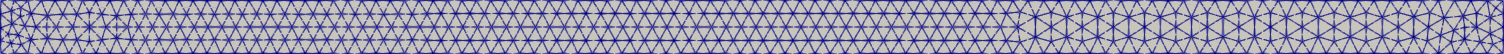
\includegraphics[width=\linewidth]{Figuras/backwardFacingStep/malha1.png}
        \caption{Vista lateral.}
    \end{subfigure}
    \begin{subfigure}{\textwidth}
        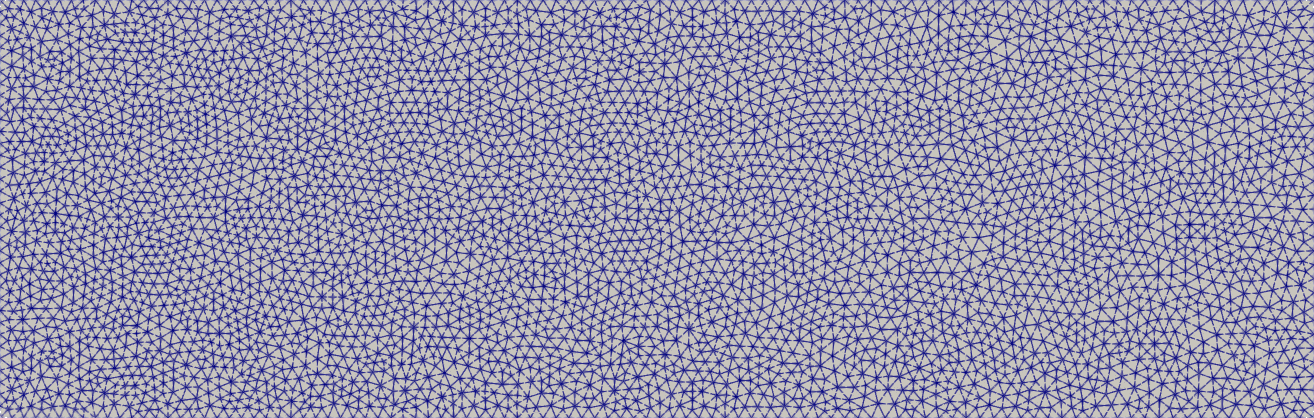
\includegraphics[width=\linewidth]{Figuras/backwardFacingStep/malha2.png}
        \caption{Vista superior.}
    \end{subfigure}
    \\Fonte: Presente trabalho (\the\year).
    \label{fig:step-mesh}
\end{figure}

O número de Reynolds do problema analisado é obtido a partir da equação \eqref{eq:ReyBFS}:

\begin{equation}
    \Rey=\frac{\rho u_\mathrm{medio}(2h)}{\mu}\text{,}
    \label{eq:ReyBFS}
\end{equation}

\noindent sendo $u_\mathrm{medio}=1,0$ a velocidade média na região de entrada do duto. Assim, sendo $\rho=1,0$, considera-se os valores de viscosidade dinâmica $\mu=0,02$, $5,1414\times10^{-3}$ e $2,0\times10^{-3}$, de modo a obter números de Reynolds de 100, 389 e 1000, respectivamente. O passo de tempo foi de $\Delta t=0,1$ e a simulação foi mantida até que a estacionariedade do fluxo fosse alcançada, sendo o esquema de integração temporal obtido a partir de $\rhoinf=0,0$. A simulação com elementos P2P2 foi estabilizada a partir da formulação SUPG/PSPG, enquanto a simulação P2P1 não foi estabilizada para $\Rey=100$ e $389$, uma vez que a simulação se tornou instável para $\Rey=1000$, sendo, portanto, necessária a aplicação de uma estabilização SUPG nesse caso.

Além disso, uma simulação bidimensional foi conduzida para o $\Rey=1000$, uma vez que \citeonline{chiang1999numerical} observaram uma discrepância entre os valores de simulações bidimensionais e tridimensionais para esse número de Reynolds. Como mencionado pelos autores, essa diferença se dá pela influência da parede aderente nos resultados, o que não é capturada pela simulação bidimensional.

A malha utilizada para a simulação bidimensional foi construída a partir de elementos P2P2 de tamanho 0,5 na região de entrada do duto e 0,6 na região de saída. Assim obtém-se uma malha com 836 elementos finitos e 1883 nós, resultando em 5649 graus de liberdade.

A Figura \ref{fig:BFSvel} apresenta os perfis de velocidade para diferentes distâncias ao longo da linha de fluxo para as três simulações conduzidas. Já a Figura \ref{fig:BFSpre} apresenta as distribuições de pressão ao longo do fundo e do topo do duto para as três simulações.

\begin{figure}[h!]
    \centering
    \caption{Escoamento em degrau invertido - Perfis de velocidade.}
    \begin{subfigure}{0.9\textwidth}
        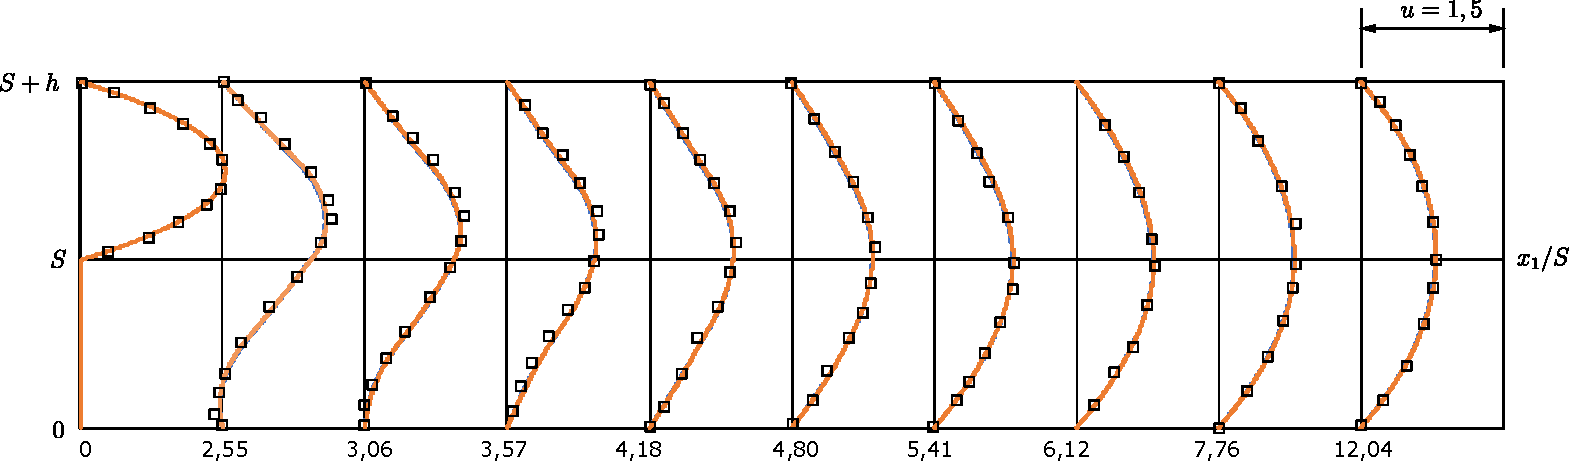
\includegraphics[width=\linewidth]{Figuras/backwardFacingStep/Re100.pdf}
        \caption{$\Rey=100$}
    \end{subfigure}
    \begin{subfigure}{0.9\textwidth}
        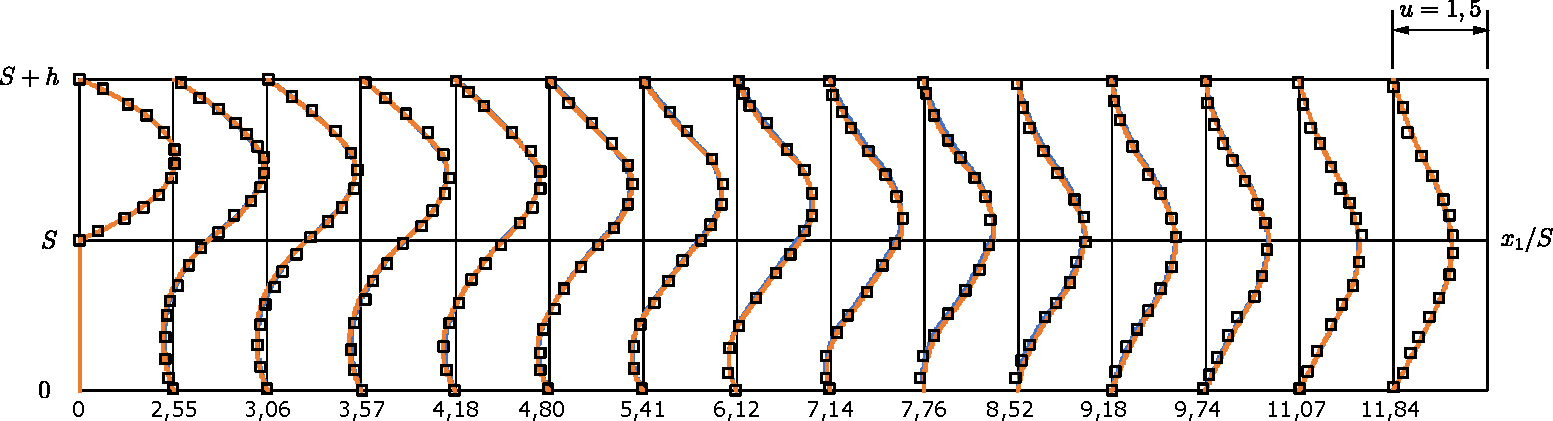
\includegraphics[width=\linewidth]{Figuras/backwardFacingStep/Re389.pdf}
        \caption{$\Rey=389$}
    \end{subfigure}
    \begin{subfigure}{0.9\textwidth}
        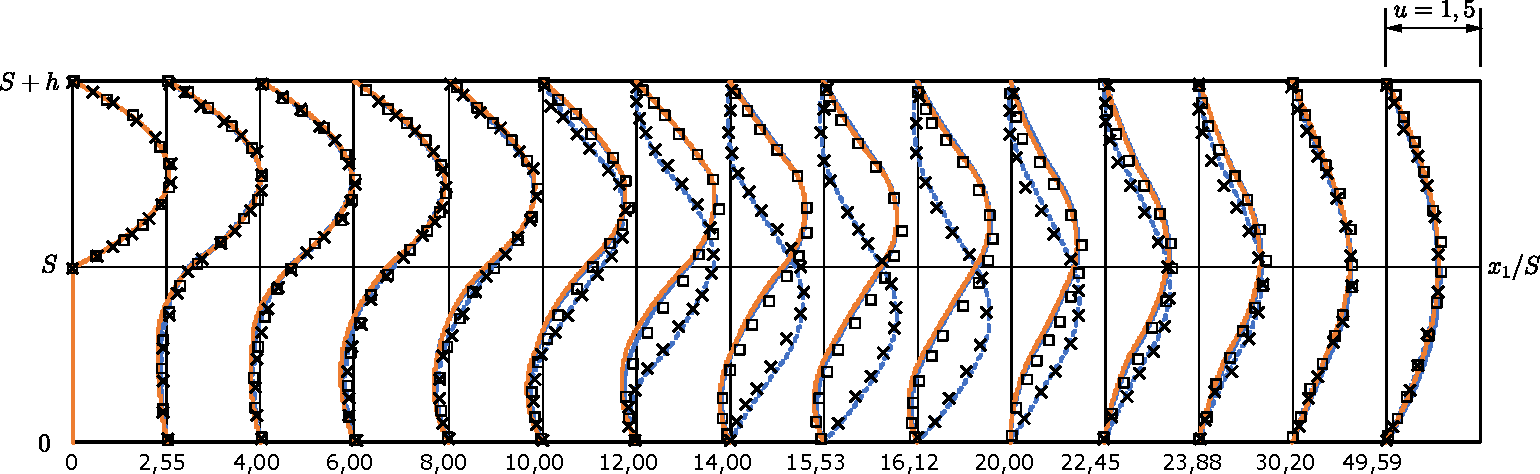
\includegraphics[width=\linewidth]{Figuras/backwardFacingStep/Re1000.pdf}
        \caption{$\Rey=1000$}
    \end{subfigure}
    \begin{subfigure}{0.3\textwidth}
        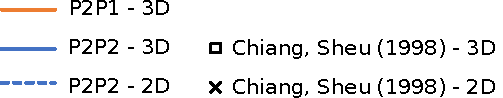
\includegraphics[width=\linewidth]{Figuras/backwardFacingStep/legenda.pdf}
    \end{subfigure}
    \\Fonte: Presente trabalho (\the\year).
    \label{fig:BFSvel}
\end{figure}

\begin{figure}[h!]
    \centering
    \caption{Escoamento em degrau invertido - Distribuição de pressões.}
    \begin{subfigure}{0.65\textwidth}
        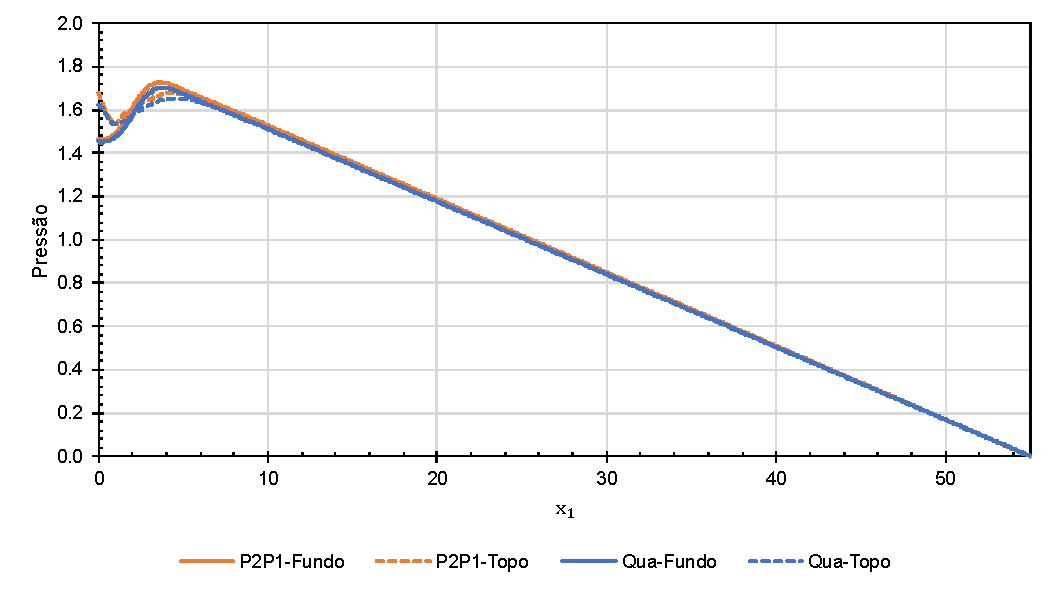
\includegraphics[width=\linewidth]{Figuras/backwardFacingStep/pre100.pdf}
        \caption{$\Rey=100$}
    \end{subfigure}
    \begin{subfigure}{0.65\textwidth}
        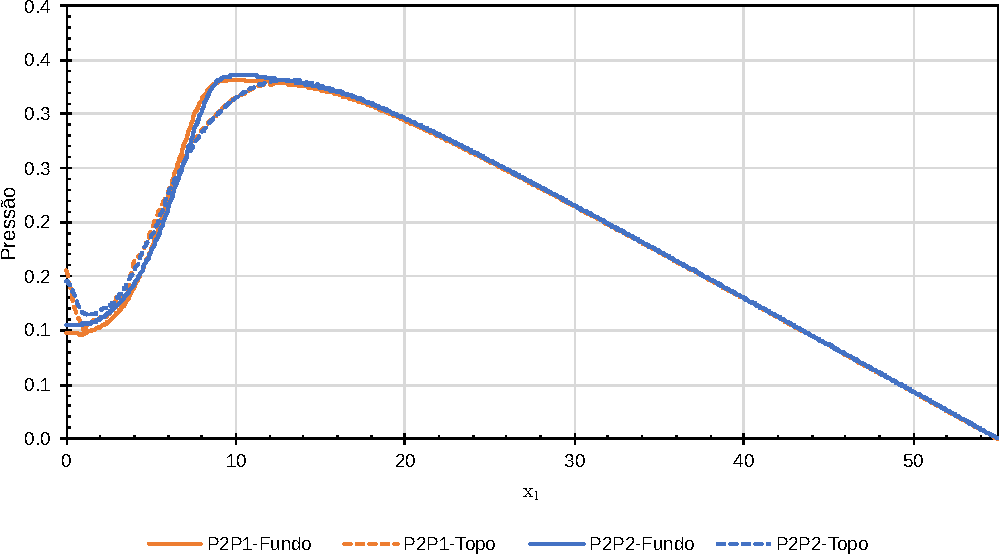
\includegraphics[width=\linewidth]{Figuras/backwardFacingStep/pre389.pdf}
        \caption{$\Rey=389$}
    \end{subfigure}
    \begin{subfigure}{0.65\textwidth}
        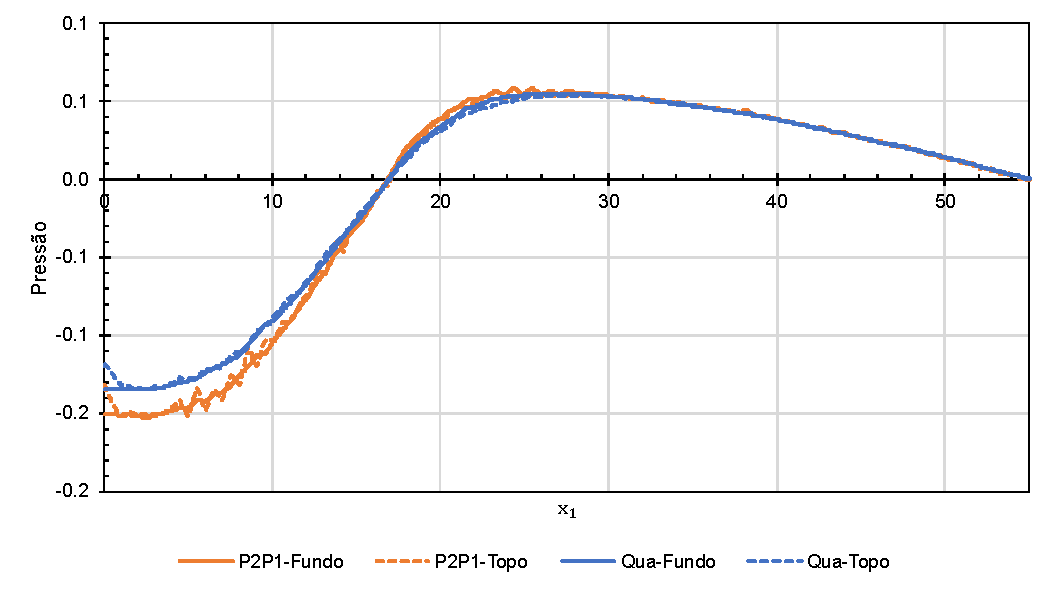
\includegraphics[width=\linewidth]{Figuras/backwardFacingStep/pre1000.pdf}
        \caption{$\Rey=1000$}
    \end{subfigure}
    \\Fonte: Presente trabalho (\the\year).
    \label{fig:BFSpre}
\end{figure}

Outra simulação realizada trata-se do problema bidimensional com $S=1$ e $\Rey=800$, onde os autores observaram os perfis de velocidade para as distâncias $x_1=14$ e $x_1=30$, além da distribuição de pressões ao longo do fundo e do topo do canal. Como a pressão de estagnação do problema simulado é nula na face de saída do duto, foi apenas adicionada uma pressão constante nos resultados de referência para fins de comparação, de forma que as pressões sejam equivalentes nesse ponto especificado. As Figuras \ref{fig:BFS800-vel} e \ref{fig:BFS800-pre} apresentam os resultados obtidos para a simulação bidimensional.

\begin{figure}[h!]
    \centering
    \caption{Escoamento em degrau invertido - Perfis de velocidade para $\Rey=800$.}
    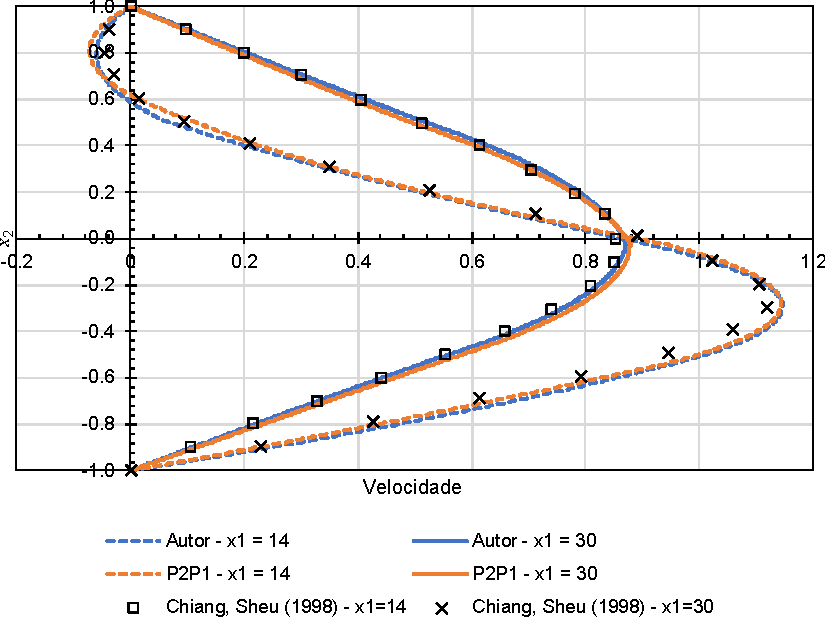
\includegraphics[width=.6\linewidth]{Figuras/backwardFacingStep/resultado2D-2.pdf}
    \\Fonte: Presente trabalho (\the\year).
    \label{fig:BFS800-vel}
\end{figure}

\begin{figure}[h!]
    \centering
    \caption{Escoamento em degrau invertido - Distribuição de pressões para $\Rey=800$.}
    \includegraphics[width=.6\linewidth]{Figuras/backwardFacingStep/resultado2D-1.pdf}
    \\Fonte: Presente trabalho (\the\year).
    \label{fig:BFS800-pre}
\end{figure}

Assim, percebe-se que, em relação ao campo de velocidade, todas as simulações possuíram resultados satisfatórios em todos os números de Reynolds analisados, tanto em simulações bidimensionais quanto tridimensionais. No entanto, para o campo de pressão, observa-se que os elementos P2P1 apresentaram oscilações espúrias, principalmente próximo à face de entrada, o que não é observado na simulação estabilizada por PSPG.

%==================================================================================================
\subsection{Escoamento sobre cilindro} \label{ex:cylinder}
%==================================================================================================

Para o seguinte problema considerou-se um cilindro circular de raio $R=0,5$ em um domínio retangular $\Omega=[0,112R]\times[0,100R]$, sendo o centro do cilindro posicionado sobre o ponto $(36,50)R$. As condições de contorno consideradas foram de entrada na face esquerda ($x_1=0$) do domínio ($\BB{u}=\{u_\infty,0\}^T$) e condição de velocidade vertical nula nas faces inferior e superior ($u_2=0$ em $x_2=0$ e $x_2=100R$). Como condição inicial aplicou-se uma velocidade $\BB{u}=\{u_\infty,0\}^T$ em todo o domínio. A densidade do fluido foi de $\rho=1,0$ e a velocidade $u_\infty=1,0$. A viscosidade dinâmica do fluido foi de $\nu=0,01$, $\nu=6,6667\times10^{-3}$ e $\nu=5\times10^{-3}$, de forma a se obter $\Rey=100$, $\Rey=150$ e $\Rey=200$, respectivamente.

Para a simulação numérica considerou-se a malha apresentada na Figura \ref{fig:cyl-mesh}, a qual possui 4656 elementos finitos. Assim, estudou-se o escoamento nas simulações apresentadas na Tabela \ref{tab:cyl-sim}. O intervalo de tempo foi de $t\in[0,200]$ com passos de $\Delta t=0,1$.

\begin{figure}[h!]
    \centering
    \caption{Escoamento sobre cilindro - Malha utilizada.}
    \includegraphics[width=\linewidth]{Figuras/cylinder/analise2/mesh.png}
    \\Fonte: Presente trabalho (\the\year).
    \label{fig:cyl-mesh}
\end{figure}

\begin{table}[h!]
    \centering
    \caption{Simulações conduzidas para o problema de escoamento sobre um cilindro.}
    \begin{tabular}{llllc}
        \hline
        Nome & Modelo & Elemento & Estabilização & Número de DOF \\\hline
        Sim1 & -      & P2P1     & -             & 21417         \\
        Sim2 & -      & P2P2     & SUPG/PSPG     & 28494         \\
        Sim3 & -      & P2P2     & VMS           & 28494         \\
        Sim4 & LES    & P2P1     & -             & 21417         \\
        Sim5 & LES    & P2P2     & VMS           & 28494         \\\hline
    \end{tabular}
    \\Fonte: Presente trabalho (\the\year).
    \label{tab:cyl-sim}
\end{table}

Para análise dos resultados determinou-se os coeficientes de arrasto (\textit{Drag} - $C_D$) e de sustentação (\textit{Lift} - $C_L$), dados respectivamente por:

\begin{subequations}
    \begin{equation}
        C_D=\frac{2F_D}{\rho\norm{\BB{u}_\infty}^2L}\text{ e}
    \end{equation}
    \begin{equation}
        C_L=\frac{2F_L}{\rho\norm{\BB{u}_\infty}^2L}\text{,}
    \end{equation}
\end{subequations}

\noindent em que $F_D$ e $F_L$ são as forças de arrasto e de sustentação, calculados como:

\begin{subequations}
    \begin{equation}
        F_D=\int_{\Gamma_S}{\sigma_{1j}n_jd\Gamma_S}\text{ e}
    \end{equation}
    \begin{equation}
        F_L=\int_{\Gamma_S}{\sigma_{2j}n_jd\Gamma_S}\text{,}
    \end{equation}
\end{subequations}

\noindent sendo $\Gamma_S$ a fronteira do cilindro e $\BB{n}$ o vetor normal à $\Gamma_S$.

Outro parâmetro possível de se verificar é o número de Strouhal ($\Str$), que se trata de um número adimensional que busca relacionar a frequência de oscilação devido à formação de vórtices e a velocidade do fluido. Esse parâmetro pode ser determinado por:

\begin{equation}
    \Str=\frac{f_vL}{\norm{\BB{u}_\infty}}\text{,}
\end{equation}

\noindent sendo $f_v$ a frequência de desprendimento de vórtices.

As Figuras \ref{fig:cyl-Cd} e \ref{fig:cyl-Cl} apresentam os coeficientes de arrasto e de sustentação obtidos em todas as simulações, respectivamente.

\begin{figure}[h!]
    \centering
    \caption{Escoamento sobre cilindro - Coeficiente de arrasto ao longo do tempo.}
    \begin{subfigure}{\textwidth}
        \includegraphics[width=\linewidth]{Figuras/cylinder/analise3/Cd-100.pdf}
        \caption{$\Rey=100$}
    \end{subfigure}
    \begin{subfigure}{\textwidth}
        \includegraphics[width=\linewidth]{Figuras/cylinder/analise3/Cd-150.pdf}
        \caption{$\Rey=150$}
    \end{subfigure}
    \begin{subfigure}{\textwidth}
        \includegraphics[width=\linewidth]{Figuras/cylinder/analise3/Cd-200.pdf}
        \caption{$\Rey=200$}
    \end{subfigure}
    \begin{subfigure}{.8\textwidth}
        \includegraphics[width=\linewidth]{Figuras/cylinder/legenda.pdf}
    \end{subfigure}
    \\Fonte: Presente trabalho (\the\year).
    \label{fig:cyl-Cd}
\end{figure}
\newpage

\begin{figure}[h!]
    \centering
    \caption{Escoamento sobre cilindro - Coeficiente de sustentação ao longo do tempo.}
    \begin{subfigure}{\textwidth}
        \includegraphics[width=\linewidth]{Figuras/cylinder/analise3/Cl-100.pdf}
        \caption{$\Rey=100$}
    \end{subfigure}
    \begin{subfigure}{\textwidth}
        \includegraphics[width=\linewidth]{Figuras/cylinder/analise3/Cl-150.pdf}
        \caption{$\Rey=150$}
    \end{subfigure}
    \begin{subfigure}{\textwidth}
        \includegraphics[width=\linewidth]{Figuras/cylinder/analise3/Cl-200.pdf}
        \caption{$\Rey=200$}
    \end{subfigure}
    \begin{subfigure}{.8\textwidth}
        \includegraphics[width=\linewidth]{Figuras/cylinder/legenda.pdf}
    \end{subfigure}
    \\Fonte: Presente trabalho (\the\year).
    \label{fig:cyl-Cl}
\end{figure}
\newpage

Os valores dos coeficientes de arrasto e de sustentação após o escoamento atingir o equilíbrio dinâmico, assim como o número de Strouhal e valores de referência, são apresentados nas Tabelas \ref{tab:cyl-res100} a \ref{tab:cyl-res200}.

\begin{table}[h!]
    \centering
    \caption{Escoamento sobre cilindro - Valores dos coeficientes e número de Strouhal para $\Rey=100$.}
    \begin{tabular}{lcccc}
        \hline
        Simulação                          & $C_D$             & $C_L$       & $\Str$   \\\hline
        Sim1                               & $1,3458\pm0,0095$ & $\pm0,3283$ & $0,1642$ \\
        Sim2                               & $1,3488\pm0,0094$ & $\pm0,3255$ & $0,1647$ \\
        Sim3                               & $1,3480\pm0,0095$ & $\pm0,3279$ & $0,1650$ \\
        Sim4                               & $1,3445\pm0,0093$ & $\pm0,3264$ & $0,1639$ \\
        Sim5                               & $1,3466\pm0,0094$ & $\pm0,3259$ & $0,1646$ \\\hline
        \citeonline{fernandes2020tecnica}  & $1,3700\pm0,0098$ & $\pm0,3422$ & $0,165$  \\
        \citeonline{najafi2012meshless}    & $1,47$            & $\pm0,38$   &          \\
        \citeonline{ji2012novel}           & $1,4643\pm0,0107$ & $\pm0,3351$ & $0,1675$ \\
        \citeonline{liu1998preconditioned} & $1,350\pm0,012$   & $\pm0,339$  & $0,165$  \\\hline
    \end{tabular}
    \\Fonte: Presente trabalho (\the\year).
    \label{tab:cyl-res100}
\end{table}

\begin{table}[h!]
    \centering
    \caption{Escoamento sobre cilindro - Valores dos coeficientes e número de Strouhal para $\Rey=150$.}
    \begin{tabular}{lcccc}
        \hline
        Simulação                          & $C_D$             & $C_D$       & $\Str$   \\\hline
        Sim1                               & $1,3309\pm0,0262$ & $\pm0,5218$ & $0,1848$ \\
        Sim2                               & $1,3384\pm0,0263$ & $\pm0,5231$ & $0,1852$ \\
        Sim3                               & $1,3369\pm0,0265$ & $\pm0,5253$ & $0,1855$ \\
        Sim4                               & $1,3283\pm0,0257$ & $\pm0,5184$ & $0,1843$ \\
        Sim5                               & $1,3358\pm0,0259$ & $\pm0,5196$ & $0,1847$ \\\hline
        \citeonline{najafi2012meshless}    & $1,45$            & $\pm0,56$   &          \\
        \citeonline{ji2012novel}           & $1,4463\pm0,0261$ & $\pm0,5043$ & $0,1837$ \\
        \citeonline{liu1998preconditioned} & $1,334\pm0,030$   & $\pm0,530$  & $0,182$  \\\hline
    \end{tabular}
    \\Fonte: Presente trabalho (\the\year).
    \label{tab:cyl-res150}
\end{table}

\begin{table}[h!]
    \centering
    \caption{Escoamento sobre cilindro - Valores dos coeficientes e número de Strouhal para $\Rey=200$.}
    \begin{tabular}{lcccc}
        \hline
        Simulação                          & $C_D$             & $C_L$       & $\Str$   \\\hline
        Sim1                               & $1,3409\pm0,0450$ & $\pm0,6833$ & $0,1987$ \\
        Sim2                               & $1,3527\pm0,0456$ & $\pm0,6874$ & $0,1998$ \\
        Sim3                               & $1,3506\pm0,0457$ & $\pm0,6892$ & $0,2001$ \\
        Sim4                               & $1,3374\pm0,0442$ & $\pm0,6784$ & $0,1980$ \\
        Sim5                               & $1,3490\pm0,0449$ & $\pm0,6825$ & $0,1990$ \\\hline
        \citeonline{fernandes2020tecnica}  & $1,3787\pm0,0476$ & $\pm0,7134$ & $0,195$  \\
        \citeonline{najafi2012meshless}    & $1,46$            & $\pm0,72$   &          \\
        \citeonline{ji2012novel}           & $1,4372\pm0,0417$ & $\pm0,6272$ & $0,1963$ \\
        \citeonline{liu1998preconditioned} & $1,31\pm0,049$    & $\pm0,69$   & $0,192$  \\\hline
    \end{tabular}
    \\Fonte: Presente trabalho (\the\year).
    \label{tab:cyl-res200}
\end{table}

Assim, observa-se que todos os valores estão próximos aos valores de referência, sendo que as simulações baseadas em elementos P2P1 apresentaram valores ligeiramente inferiores aos demais conforme o número de Reynolds aumenta. A mínima diferença observada entre os valores calculados em uma simulação sem LES e aquela que em simulação com LES deve-se ao fato do número de Reynolds ser muito baixo, pois, como apontado por \citeonline{fernandes2020tecnica}, esse tipo de escoamento (com $\Rey$ entre 50 e 200) apresenta a formação de vórtices laminares, denominada de esteira de Von Kárman.

Em seguida partiu-se para uma análise com a consideração de uma malha mais grosseira, a qual é apresentada na Figura \ref{fig:cyl-mesh2}. A malha utilizada para a simulação foi construída a partir de elementos triangulares, possuindo 5004 graus de liberdade para a simulação de elementos P2P2 e 3771 para a simulação de elementos P2P1. Os valores dos coeficientes de arrasto e de sustentação são apresentados nas Figuras \ref{fig:cyl-Cd2} e \ref{fig:cyl-Cl2}, respectivamente. A linha de referência é considerada como a obtida pela simulação LES-VMS da malha fina.

\begin{figure}[h!]
    \centering
    \caption{Escoamento sobre cilindro - Malha utilizada para simulação com malha mais grosseira.}
    \includegraphics[width=.75\linewidth]{Figuras/cylinder/coarse/mesh.png}
    \\Fonte: Presente trabalho (\the\year).
    \label{fig:cyl-mesh2}
\end{figure}

\begin{figure}[h!]
    \centering
    \caption{Escoamento sobre cilindro - Coeficiente de arrasto ao longo do tempo para malha mais grosseira.}
    \begin{subfigure}{\textwidth}
        \centering
        \includegraphics[width=.85\linewidth]{Figuras/cylinder/coarse/Cd100.pdf}
        \caption{$\Rey=100$}
    \end{subfigure}
    \begin{subfigure}{\textwidth}
        \centering
        \includegraphics[width=.85\linewidth]{Figuras/cylinder/coarse/Cd150.pdf}
        \caption{$\Rey=150$}
    \end{subfigure}
    \begin{subfigure}{\textwidth}
        \centering
        \includegraphics[width=.85\linewidth]{Figuras/cylinder/coarse/Cd200.pdf}
        \caption{$\Rey=200$}
    \end{subfigure}
    \begin{subfigure}{.8\textwidth}
        \includegraphics[width=\linewidth]{Figuras/cylinder/legenda2.pdf}
    \end{subfigure}
    \\Fonte: Presente trabalho (\the\year).
    \label{fig:cyl-Cd2}
\end{figure}

\begin{figure}[h!]
    \centering
    \caption{Escoamento sobre cilindro - Coeficiente de sustentação ao longo do tempo para malha mais grosseira.}
    \begin{subfigure}{\textwidth}
        \includegraphics[width=\linewidth]{Figuras/cylinder/coarse/Cl100.pdf}
        \caption{$\Rey=100$}
    \end{subfigure}
    \begin{subfigure}{\textwidth}
        \includegraphics[width=\linewidth]{Figuras/cylinder/coarse/Cl150.pdf}
        \caption{$\Rey=150$}
    \end{subfigure}
    \begin{subfigure}{\textwidth}
        \includegraphics[width=\linewidth]{Figuras/cylinder/coarse/Cl200.pdf}
        \caption{$\Rey=200$}
    \end{subfigure}
    \begin{subfigure}{.8\textwidth}
        \includegraphics[width=\linewidth]{Figuras/cylinder/legenda2.pdf}
    \end{subfigure}
    \\Fonte: Presente trabalho (\the\year).
    \label{fig:cyl-Cl2}
\end{figure}

Os valores dos coeficientes de arrasto e de sustentação após o escoamento atingir o equilíbrio dinâmico, assim como o número de Strouhal e valores obtidos na simulação com malha fina, são apresentados na Tabela \ref{tab:cyl-comp100} a \ref{tab:cyl-comp200}.

\begin{table}[h!]
    \centering
    \caption{Escoamento sobre cilindro - Comparação de $C_D$, $C_L$ e $\Str$ para $\Rey=100$.}
    \begin{tabular}{lcccccc}
        \hline
        \multirow{2}{*}{Simulação} & \multicolumn{3}{c}{Malha 1} & \multicolumn{3}{c}{Malha 2}                                                         \\\cline{2-7}
                                   & $C_D$                       & $C_L$                       & $\Str$   & $C_D$             & $C_L$       & $\Str$   \\\hline
        Sim1                       & $1,3458\pm0,0095$           & $\pm0,3283$                 & $0,1642$ & $1,1913\pm0,0120$ & $\pm0,2966$ & $0,1464$ \\
        Sim2                       & $1,3488\pm0,0094$           & $\pm0,3255$                 & $0,1647$ & $1,3502\pm0,0128$ & $\pm0,3637$ & $0,1614$ \\
        Sim3                       & $1,3480\pm0,0095$           & $\pm0,3279$                 & $0,1650$ & $1,3320\pm0,0136$ & $\pm0,3759$ & $0,1621$ \\
        Sim4                       & $1,3445\pm0,0093$           & $\pm0,3264$                 & $0,1639$ & $1,1832\pm0,0103$ & $\pm0,2683$ & $0,1442$ \\
        Sim5                       & $1,3466\pm0,0094$           & $\pm0,3259$                 & $0,1646$ & $1,3210\pm0,0121$ & $\pm0,3527$ & $0,1589$ \\\hline
    \end{tabular}
    \\Fonte: Presente trabalho (\the\year).
    \label{tab:cyl-comp100}
\end{table}

\begin{table}[h!]
    \centering
    \caption{Escoamento sobre cilindro - Comparação de $C_D$, $C_L$ e $\Str$ para $\Rey=150$.}
    \begin{tabular}{lcccccc}
        \hline
        \multirow{2}{*}{Simulação} & \multicolumn{3}{c}{Malha 1} & \multicolumn{3}{c}{Malha 2}                                                         \\\cline{2-7}
                                   & $C_D$                       & $C_L$                       & $\Str$   & $C_D$             & $C_L$       & $\Str$   \\\hline
        Sim1                       & $1,3309\pm0,0262$           & $\pm0,5218$                 & $0,1848$ & $1,2101\pm0,0416$ & $\pm0,5879$ & $0,1661$ \\
        Sim2                       & $1,3384\pm0,0263$           & $\pm0,5231$                 & $0,1852$ & $1,3822\pm0,0364$ & $\pm0,5915$ & $0,1821$ \\
        Sim3                       & $1,3369\pm0,0265$           & $\pm0,5253$                 & $0,1855$ & $1,3660\pm0,0378$ & $\pm0,6059$ & $0,1822$ \\
        Sim4                       & $1,3283\pm0,0257$           & $\pm0,5184$                 & $0,1843$ & $1,1952\pm0,0337$ & $\pm0,5433$ & $0,1626$ \\
        Sim5                       & $1,3358\pm0,0259$           & $\pm0,5196$                 & $0,1847$ & $1,3491\pm0,0346$ & $\pm0,5768$ & $0,1779$ \\\hline
    \end{tabular}
    \\Fonte: Presente trabalho (\the\year).
    \label{tab:cyl-comp150}
\end{table}

\begin{table}[h!]
    \centering
    \caption{Escoamento sobre cilindro - Comparação de $C_D$, $C_L$ e $\Str$ para $\Rey=200$.}
    \begin{tabular}{lcccccc}
        \hline
        \multirow{2}{*}{Simulação} & \multicolumn{3}{c}{Malha 1} & \multicolumn{3}{c}{Malha 2}                                                         \\\cline{2-7}
                                   & $C_D$                       & $C_L$                       & $\Str$   & $C_D$             & $C_L$       & $\Str$   \\\hline
        Sim1                       & $1,3409\pm0,0450$           & $\pm0,6833$                 & $0,1987$ & $1,2118\pm0,0672$ & $\pm0,7190$ & $0,1776$ \\
        Sim2                       & $1,3527\pm0,0456$           & $\pm0,6874$                 & $0,1998$ & $1,4232\pm0,7477$ & $\pm0,7477$ & $0,1947$ \\
        Sim3                       & $1,3506\pm0,0457$           & $\pm0,6892$                 & $0,2001$ & $1,4108\pm0,7646$ & $\pm0,7646$ & $0,1943$ \\
        Sim4                       & $1,3374\pm0,0442$           & $\pm0,6784$                 & $0,1980$ & $1,1997\pm0,6768$ & $\pm0,6768$ & $0,1735$ \\
        Sim5                       & $1,3490\pm0,0449$           & $\pm0,6825$                 & $0,1990$ & $1,3887\pm0,7283$ & $\pm0,7283$ & $0,1894$ \\\hline
    \end{tabular}
    \\Fonte: Presente trabalho (\the\year).
    \label{tab:cyl-comp200}
\end{table}

Como pode se observar, os valores obtidos a partir de elementos P2P1 tiveram valores muito abaixo do esperado, principalmente para o coeficiente de arrasto, independentemente da aplicação do LES. Já os valores obtidos a partir de elementos P2P2 apresentaram valores mais próximos aos obtidos na simulação com malha mais fina, em que a aplicação do LES se mostrou eficiente para descrever os coeficientes de arrasto e sustentação a partir de $\Rey=150$. Já o número de Strouhal foi levemente amortecido devido à aplicação do modelo.

%Comparando-se os números de Strouhal calculados com aqueles obtidos por \citeonline{fernandes2020tecnica}, que obteve, para a mesma geometria de domínio e mesmas condições de contorno, um $\Str=0,165$ e amplitude do coeficiente de sustentação de 0,3422, \citeonline{tezduyar1992incompressible}, os quais verificaram $\Str$ entre 0,166 e 0,170, \citeonline{najafi2012meshless}, com valor de 0,182, e \citeonline{codina2006numerical}, com valores entre 0,177 e 0,184. As variações observadas entre os números de Strouhal dos diferentes autores podem ser devidas às diferenças nas dimensões dos domínios utilizados, assim como as diferentes condições de contorno aplicadas por cada um. No entanto ainda observa-se que em todos os casos os valores calculados nas simulações ainda são bem próximos. A mínima diferença observada entre os valores calculados em uma simulação DNS e aquela que em simulação LES deve-se ao fato do número de Reynolds ser muito baixo, pois, como apontado por \citeonline{fernandes2020tecnica}, esse tipo de escoamento (com $\Rey$ entre 50 e 200) apresenta a formação de vórtices laminares, denominada de esteira de Von Kárman. Para uma verificação mais precisa dessa influência, deve-se partir para uma análise tridimensional com número de Reynolds superiores à 200.

%Vale observar ainda que a simulação VMS linear apresentou um amortecimento menor em relação ao início das oscilações, porém converge para valores muito próximos ao quadrático ao longo do tempo. Já a simulação LES inicia sua oscilação próxima ao VMS quadrático, entretanto com uma média de oscilação menor que a do VMS, em especial ao se observar o coeficiente de arrasto. Tal efeito pode ser devido ao relatado por \citeonline{germano1991dynamic,hughes2000large}, que apontam a ocorrência de um amortecimento excessivo provocado pelo tensor SGS de Smagorinsky.
\begin{comment}
\begin{figure}[h!]
    \centering
    \caption{Campos de velocidade e de pressões no instante $t=120$ para elemento de aproximação linear.}
    \begin{subfigure}{\textwidth}
        \begin{subfigure}{\textwidth}\centering
            \begin{subfigure}{.42\textwidth}
                \caption*{Campo de velocidade.}
                \includegraphics[width=\linewidth]{Figuras/cylinder/analise2/lu.png}
            \end{subfigure}
            \begin{subfigure}{.42\textwidth}
                \caption*{Campo de pressões.}
                \includegraphics[width=\linewidth]{Figuras/cylinder/analise2/lp.png}
            \end{subfigure}
        \end{subfigure}
    \end{subfigure}
    \begin{subfigure}{\textwidth}\centering
        \begin{subfigure}{.49\textwidth}
            \includegraphics[width=\linewidth]{Figuras/cylinder/analise2/none-Lin-u.png}
        \end{subfigure}
        \begin{subfigure}{.49\textwidth}
            \includegraphics[width=\linewidth]{Figuras/cylinder/analise2/none-Lin-p.png}
        \end{subfigure}
        \caption{Sem modelo}
    \end{subfigure}
    \begin{subfigure}{\textwidth}\centering
        \begin{subfigure}{.49\textwidth}
            \includegraphics[width=\linewidth]{Figuras/cylinder/analise2/LES-Lin-u.png}
        \end{subfigure}
        \begin{subfigure}{.49\textwidth}
            \includegraphics[width=\linewidth]{Figuras/cylinder/analise2/LES-Lin-p.png}
        \end{subfigure}
        \caption{LES}
    \end{subfigure}
    \begin{subfigure}{\textwidth}\centering
        \begin{subfigure}{.49\textwidth}
            \includegraphics[width=\linewidth]{Figuras/cylinder/analise2/VMS-Lin-u.png}
        \end{subfigure}
        \begin{subfigure}{.49\textwidth}
            \includegraphics[width=\linewidth]{Figuras/cylinder/analise2/VMS-Lin-p.png}
        \end{subfigure}
        \caption{VMS}
    \end{subfigure}
    \\Fonte: Presente trabalho (\the\year).
    \label{fig:vel-pre-Lin}
\end{figure}
\newpage

\begin{figure}[h!]
    \centering
    \caption{Campos de velocidade e de pressões no instante $t=120$ para elemento de aproximação quadrática.}
    \begin{subfigure}{\textwidth}
        \begin{subfigure}{\textwidth}\centering
            \begin{subfigure}{.42\textwidth}
                \caption*{Campo de velocidade.}
                \includegraphics[width=\linewidth]{Figuras/cylinder/analise2/lu.png}
            \end{subfigure}
            \begin{subfigure}{.42\textwidth}
                \caption*{Campo de pressões.}
                \includegraphics[width=\linewidth]{Figuras/cylinder/analise2/lp.png}
            \end{subfigure}
        \end{subfigure}
    \end{subfigure}
    \begin{subfigure}{\textwidth}\centering
        \begin{subfigure}{.49\textwidth}
            \includegraphics[width=\linewidth]{Figuras/cylinder/analise2/none-Qua-u.png}
        \end{subfigure}
        \begin{subfigure}{.49\textwidth}
            \includegraphics[width=\linewidth]{Figuras/cylinder/analise2/none-Qua-p.png}
        \end{subfigure}
        \caption{Sem modelo}
    \end{subfigure}
    \begin{subfigure}{\textwidth}\centering
        \begin{subfigure}{.49\textwidth}
            \includegraphics[width=\linewidth]{Figuras/cylinder/analise2/LES-Qua-u.png}
        \end{subfigure}
        \begin{subfigure}{.49\textwidth}
            \includegraphics[width=\linewidth]{Figuras/cylinder/analise2/LES-Qua-p.png}
        \end{subfigure}
        \caption{LES}
    \end{subfigure}
    \begin{subfigure}{\textwidth}\centering
        \begin{subfigure}{.49\textwidth}
            \includegraphics[width=\linewidth]{Figuras/cylinder/analise2/VMS-Qua-u.png}
        \end{subfigure}
        \begin{subfigure}{.49\textwidth}
            \includegraphics[width=\linewidth]{Figuras/cylinder/analise2/VMS-Qua-p.png}
        \end{subfigure}
        \caption{VMS}
    \end{subfigure}
    \\Fonte: Presente trabalho (\the\year).
    \label{fig:vel-pre-Qua}
\end{figure}
\newpage

\begin{figure}[h!]
    \centering
    \caption{Campos de velocidade e de pressões no instante $t=120$ para elemento Taylor-Hood P2P1.}
    \begin{subfigure}{\textwidth}
        \begin{subfigure}{\textwidth}\centering
            \begin{subfigure}{.42\textwidth}
                \caption*{Campo de velocidade.}
                \includegraphics[width=\linewidth]{Figuras/cylinder/analise2/lu.png}
            \end{subfigure}
            \begin{subfigure}{.42\textwidth}
                \caption*{Campo de pressões.}
                \includegraphics[width=\linewidth]{Figuras/cylinder/analise2/lp.png}
            \end{subfigure}
        \end{subfigure}
    \end{subfigure}
    \begin{subfigure}{\textwidth}\centering
        \begin{subfigure}{.49\textwidth}
            \includegraphics[width=\linewidth]{Figuras/cylinder/analise2/none-TH-u.png}
        \end{subfigure}
        \begin{subfigure}{.49\textwidth}
            \includegraphics[width=\linewidth]{Figuras/cylinder/analise2/none-TH-p.png}
        \end{subfigure}
        \caption{Sem modelo}
    \end{subfigure}
    \begin{subfigure}{\textwidth}\centering
        \begin{subfigure}{.49\textwidth}
            \includegraphics[width=\linewidth]{Figuras/cylinder/analise2/LES-TH-u.png}
        \end{subfigure}
        \begin{subfigure}{.49\textwidth}
            \includegraphics[width=\linewidth]{Figuras/cylinder/analise2/LES-TH-p.png}
        \end{subfigure}
        \caption{LES}
    \end{subfigure}
    \begin{subfigure}{\textwidth}\centering
        \begin{subfigure}{.49\textwidth}
            \includegraphics[width=\linewidth]{Figuras/cylinder/analise2/VMS-TH-u.png}
        \end{subfigure}
        \begin{subfigure}{.49\textwidth}
            \includegraphics[width=\linewidth]{Figuras/cylinder/analise2/VMS-TH-p.png}
        \end{subfigure}
        \caption{VMS}
    \end{subfigure}
    \\Fonte: Presente trabalho (\the\year).
    \label{fig:vel-pre-TH}
\end{figure}
\newpage
\end{comment}

%==================================================================================================
\subsection{Escoamento sobre um aerofólio NACA 0012} \label{ex:NACA0012}
%==================================================================================================

O seguinte exemplo trata-se de um escoamento em torno de um aerofólio NACA 0012, cujo comprimento da corda é unitário ($L=1,0$). O domínio considerado para a simulação é apresentado na Figura \ref{fig:NACA0012}, em que o ângulo de ataque $\alpha=5^{\circ}$. O fluido possui massa específica $\rho=1,0$, viscosidade dinâmica $\mu=2\times10^{-5}$ e a velocidade de entrada é de $\BB{u}_\infty=[1,0]\trans$, resultando em o número de Reynolds de $\Rey=5\times10^4$.

\begin{figure}[h!]
    \centering
    \caption{Escoamento em torno de um aerofólio NACA 0012 - Domínio de simulação.}
    \includegraphics[width=.7\linewidth]{Figuras/NACA0012/NACA0012.pdf}
    \\Fonte: Presente trabalho (\the\year).
    \label{fig:NACA0012}
\end{figure}

O problema foi estudado em situações bidimensionais e tridimensionais, sendo simulado tanto com e sem aplicação de LES. Em ambos os casos o problema foi estabilizado a partir da estabilização SUPG/PSPG.

A malha utilizada para a simulação bidimensional foi construída a partir de elementos P2P2, com tamanho 0,01 na superfície do aerofólio, 2,5 na região de entrada e 0,5 na região de saída. Assim obtém-se uma malha com 5247 elementos finitos, tendo 10817 nós, resultando em 32451 graus de liberdade (conforme ilustrado na Figura \ref{fig:NACA0012-mesh2D}). O intervalo de tempo utilizado foi de $t\in[0,100]$ com passos de $\Delta t=0,01$.

\begin{figure}[h!]
    \centering
    \caption{Escoamento em torno de um aerofólio NACA 0012 - Malha bidimensional.}
    \includegraphics[width=.7\linewidth]{Figuras/NACA0012/mesh2D.png}
    \\Fonte: Presente trabalho (\the\year).
    \label{fig:NACA0012-mesh2D}
\end{figure}

Já para a simulação tridimensional, considerou-se uma espessura de 0,25 para o domínio, sendo admitida uma condição simétrica nas faces $x_3=0,00$ e $x_3=0,25$. Além disso, aumentou-se o refinamento da malha na região de entrada e de saída para 0,75 e 0,5, respectivamente. Assim, a malha possui 161540 elementos finitos, tendo 248298 nós, resultando em 993192 graus de liberdade (conforme ilustrado na Figura \ref{fig:NACA0012-mesh3D}). O intervalo de tempo utilizado foi de $t\in[0,15]$ com passos de $\Delta t=0,01$.

\begin{figure}[h!]
    \centering
    \caption{Escoamento em torno de um aerofólio NACA 0012 - Malha tridimensional.}
    \includegraphics[width=.7\linewidth]{Figuras/NACA0012/mesh3D.png}
    \\Fonte: Presente trabalho (\the\year).
    \label{fig:NACA0012-mesh3D}
\end{figure}

Para a simulação tridimensional, observou-se que a simulação sem aplicação do LES divergiu rapidamente, enquanto a simulação com LES apresentou resultados satisfatórios. Assim, os resultados obtidos foram comparados com os apresentados no trabalho de \citeonline{lehmkuhl2011direct}, o qual observou a média temporal do coeficiente de pressão ao longo do comprimento do aerofólio (Figura \ref{fig:NACA0012-Cp}).

\begin{figure}[h!]
    \centering
    \caption{Escoamento em torno de um aerofólio NACA 0012 - Coeficiente de pressão.}
    \includegraphics[width=.7\linewidth]{Figuras/NACA0012/Cp.pdf}
    \\Fonte: Presente trabalho (\the\year).
    \label{fig:NACA0012-Cp}
\end{figure}

Assim, verifica-se que todas as simulações se aproximaram dos valores de referência, sendo a simulação LES tridimensional a que resultou na distribuição mais satisfatória. Isso se deve ao fato dos vórtices se formarem tridimensionalmente no espaço, o que torna a simulação bidimensional inapropriada para tal magnitude de $\Rey$.

Outros valores observados são referentes aos coeficientes médios de sustentação ($c_D$) e de arrasto ($c_L$), além da distância do ponto de desprendimento ($x_\mathrm{sep}$) e reanexação ($x_\mathrm{reat}$) do fluxo ao longo do aerofólio. Esses valores são apresentados na Tabela \ref{tab:NACA0012-sep-reat} em comparação com os obtidos por \citeonline{lehmkuhl2011direct} em simulação DNS.

\begin{table}[h!]
    \centering
    \caption{Escoamento em torno de um aerofólio NACA 0012 - Distância do ponto de desprendimento e reanexação.}
    \begin{tabular}{lccc}
        \hline
                          & Calculado & \citeonline{lehmkuhl2011direct} & Desvio \\\hline
        $c_D$             & 0,0405    & 0,0291                          & 0,0114 \\
        $c_L$             & 0,564     & 0,569                           & -0,005 \\
        $x_\mathrm{sep}$  & 0,1258    & 0,0645                          & 0,061  \\
        $x_\mathrm{reat}$ & 0,553     & 0,566                           & -0,013 \\\hline
    \end{tabular}
    \\Fonte: Presente trabalho (\the\year).
    \label{tab:NACA0012-sep-reat}
\end{table}

Observa-se, portanto, que todos os valores estão muito próximos aos valores de referência, apontando a boa utilização do modelo. A boa estimativa dos pontos de desprendimento e de reanexação se torna importante, pois, como apontado pelo autor, esse desprendimento forma uma bolha sobre o aerofólio, o que pode causar uma perda de sustentação, além de aumentar o arrasto, impactando diretamente na eficiência do aerofólio.

A Figura \ref{fig:NACA0012-fields} apresenta os campos de pressão, velocidade e vorticidade ($\BB{\omega}=\Ny\times\BB{u}$) em torno do aerofólio no instante $t=5,0$, para a simulação tridimensional LES.

\begin{figure}[h!]
    \centering
    \caption{Escoamento em torno de um aerofólio NACA 0012 - Campos de pressão e de velocidade.}
    \begin{subfigure}{.49\textwidth}
        \includegraphics[width=\linewidth]{Figuras/NACA0012/pressure-500.png}
        \includegraphics[width=\linewidth]{Figuras/NACA0012/pressure-colormap-500.png}
        \caption{Campo de pressão.}
    \end{subfigure}
    \begin{subfigure}{.49\textwidth}
        \includegraphics[width=\linewidth]{Figuras/NACA0012/velocity-500.png}
        \includegraphics[width=\linewidth]{Figuras/NACA0012/velocity-colormap-500.png}
        \caption{Campo de velocidade.}
    \end{subfigure}
    \begin{subfigure}{.49\textwidth}
        \includegraphics[width=\linewidth]{Figuras/NACA0012/3Dvorticity-500.png}
        \includegraphics[width=\linewidth]{Figuras/NACA0012/vorticity-colormap-500.png}
        \caption{Campo de vorticidade.}
    \end{subfigure}
    \\Fonte: Presente trabalho (\the\year).
    \label{fig:NACA0012-fields}
\end{figure}

A Figura \ref{fig:NACA0012-QCriterion} apresenta as isosuperfícies no instante $t=5,0$ onde o critério $Q$ é nulo. Esse parâmetro se trata de um invariante proposto por \citeonline{hunt1988eddies}, o qual pode ser calculado como:

\begin{equation}
    Q=\frac{\Ny\BB{u}:\NyT\BB{u}}{2}=\frac{\BB{\dDef}:\BB{\dDef}-\BB{R}:\BB{R}}{2}\text{,}
\end{equation}

\noindent em que $\BB{\dDef}$ é o tensor taxa de deformação e $\BB{R}$ é o tensor de rotação, dado como o tensor antissimétrico do gradiente de velocidades. Essa medida é comumente utilizada para identificar as regiões onde a vorticidade é dominante ($Q>0$) e onde a taxa de deformação é dominante ($Q<0$) \cite{hunt1988eddies,piomelli2000large}

\begin{figure}[h!]
    \centering
    \caption{Escoamento em torno de um aerofólio NACA 0012 - Isosuperfícies de critério $Q$ nulo.}
    \includegraphics[width=.7\linewidth]{Figuras/NACA0012/QCriterion-500.png}
    \includegraphics[width=.5\linewidth]{Figuras/NACA0012/QCriterion-colormap-500.png}
    \\Fonte: Presente trabalho (\the\year).
    \label{fig:NACA0012-QCriterion}
\end{figure}

%==================================================================================================
%=========================================CONTORNOS MÓVEIS=========================================
%==================================================================================================

%==================================================================================================
\subsection{Cilindro com deslocamento prescrito}
%==================================================================================================

O primeiro problema estudado é o cilindro com deslocamento prescrito, proposto por \citeonline{wan2007fictitious}. Nesse problema, um cilindro de raio $R=0,1\,\mathrm{m}$ encontra-se confinado em um canal definido por $\Omega=[-L/2, L/2]\times[0,H]$, com $L=2,2$ e $H=0,41$, sendo o centro do cilindro posicionado em $(0,\ 0,2)$. O movimento do cilindro ao longo do tempo é determinado por $y_1(t)=x_1+A\sin{(2\pi f t)}$, em que $A=0,25$ e $f=0,25$. As condições de contorno do problema são de paredes aderentes nas faces esquerda e direita do domínio, enquanto as faces superior e inferior são de paredes lisas. A Figura \ref{fig:moving-cylinder} apresenta o esquema do problema estudado.

\begin{figure}[h!]
    \centering
    \caption{Cilindro com deslocamento prescrito - Esquema do problema.}
    \includegraphics[width=.7\linewidth]{Figuras/moving-cylinder/moving-cilinder.pdf}
    \\Fonte: Presente trabalho (\the\year).
    \label{fig:moving-cylinder}
\end{figure}

O fluido possui viscosidade cinemática $\nu=1\times10^{-3}$, densidade $\rho=1,0$ e parte do repouso. O problema discretizado consiste na utilização de uma malha contendo 768 elementos P2P2, totalizando 1664 nós e 4992 graus de liberdade. A simulação foi estabilizada por meio de SUPG/PSPG com esquema de integração temporal dado por $\rhoinf=0,0$. O intervalo de tempo estudado é de $t\in[0,24]$ com passos de tempo $\Delta t=0,005$. A Figura \ref{fig:moving-cylinder-mesh} apresenta a configuração inicial da malha utilizada para a solução do problema.

\begin{figure}[h!]
    \centering
    \caption{Cilindro com deslocamento prescrito - Configuração inicial da malha.}
    \includegraphics[width=\linewidth]{Figuras/moving-cylinder/mesh1.png}
    \\Fonte: Presente trabalho (\the\year).
    \label{fig:moving-cylinder-mesh}
\end{figure}

Assim, a malha é deformada no início de cada passo de tempo de forma a acomodar o movimento do cilindro. Assim, calcula-se o coeficiente de arrasto ao longo do tempo e compara-se com os resultados obtidos por \citeonline{wan2007fictitious}. A Figura \ref{fig:moving-cylinder-results} apresenta a comparação entre os resultados obtidos.

\begin{figure}[h!]
    \centering
    \caption{Cilindro com deslocamento prescrito - Coeficiente de arrasto ao longo do tempo.}
    \includegraphics[width=\linewidth]{Figuras/moving-cylinder/Cd.pdf}
    \\Fonte: Presente trabalho (\the\year).
    \label{fig:moving-cylinder-results}
\end{figure}

Verifica-se que os resultados obtidos possuem boa concordância com a referência, sendo observada apenas uma pequena diferença de fase entre os resultados, o que pode ser atribuído à diferença na condição inicial do problema.

As Figuras \ref{fig:moving-t-18-9} e \ref{fig:moving-t-21} apresentam as configurações da malha nos instantes $t=18,9$ e $t=21,0$, assim como os campos de velocidade obtidos nesses instantes.

\begin{figure}[h!]
    \centering
    \caption{Cilindro com deslocamento prescrito - Configuração da malha e campo de velocidade no instante $t=18,9$.}
    \begin{subfigure}{\linewidth}
        \centering
        \includegraphics[width=\linewidth]{Figuras/moving-cylinder/m18-9.png}
        \caption{Configuração da malha.}
    \end{subfigure}
    \begin{subfigure}{\linewidth}
        \centering
        \includegraphics[width=\linewidth]{Figuras/moving-cylinder/u18-9.png}
        \caption{Campo de velocidade.}
    \end{subfigure}
    \\Fonte: Presente trabalho (\the\year).
    \label{fig:moving-t-18-9}
\end{figure}

\begin{figure}[h!]
    \centering
    \caption{Cilindro com deslocamento prescrito - Configuração da malha e campo de velocidade no instante $t=21,0$.}
    \begin{subfigure}{\linewidth}
        \centering
        \includegraphics[width=\linewidth]{Figuras/moving-cylinder/m21.png}
        \caption{Configuração da malha.}
    \end{subfigure}
    \begin{subfigure}{\linewidth}
        \centering
        \includegraphics[width=\linewidth]{Figuras/moving-cylinder/u21.png}
        \caption{Campo de velocidade.}
    \end{subfigure}
    \\Fonte: Presente trabalho (\the\year).
    \label{fig:moving-t-21}
\end{figure}

Observa-se, portanto, que o esquema de movimentação da malha foi capaz de acomodar adequadamente o movimento do cilindro, assim como apresentou resultados muito próximos aos valores de referência, apontando a boa utilização do esquema de movimentação.

%==================================================================================================
\subsection{Aerofólio com movimento de arfagem}
%==================================================================================================

O exemplo seguinte se trata de um aerofólio NACA0012 com movimento de arfagem, proposto por \citeonline{mittal1992finite}, o qual aplica esse movimento como uma rotação prescrita do aerofólio em torno de um eixo. O domínio do problema é definido por $\Omega=[-9C, 21C]\times[-10C, 10C]$, com o centro geométrico do aerofólio posicionado em $(0,0)$. Inicialmente o aerofólio possui um ângulo de ataque ($\theta$) de $10,0^\circ$ e cujo valor varia ao longo do tempo por meio de:

\begin{equation}
    \theta(t)=\frac{\theta_\mathrm{max}+\theta_\mathrm{min}}{2}-\frac{\theta_\mathrm{max}-\theta_\mathrm{min}}{2}\cos{(\omega_f t)}\text{,}
\end{equation}

\noindent em que $\theta_\mathrm{max}=30,0^\circ$ e $\theta_\mathrm{min}=10,0^\circ$ são os valores máximo e mínimo do ângulo de ataque e $\omega_f=2\pi f_f$, sendo $f_f=1,0$ a frequência de oscilação. O giro do aerofólio se dá em torno de seu centro geométrico.

As condições de contorno do problema são de entrada na face esquerda ($\BB{u}=\{u_\infty,0\}\trans$), saída à direita e condição de simetria nas faces superior e inferior. A Figura \ref{fig:rotating-airfoil} apresenta o esquema do problema estudado.

\begin{figure}[h!]
    \centering
    \caption{Aerofólio com movimento de arfagem - Esquema do problema.}
    \includegraphics[width=.8\linewidth]{Figuras/rotating-airfoil/rotating-airfoil.pdf}
    \\Fonte: Presente trabalho (\the\year).
    \label{fig:rotating-airfoil}
\end{figure}

O número de Reynolds do problema, considerando o $C=1,0$ o comprimento característico do problema e baseado na velocidade de entrada $u_\infty=1,0$, é $\Rey=1000$. Para se obter a condição inicial do problema, realizou-se uma simulação estática para cada malha, mantendo-se fixo o ângulo de ataque inicial, até que se atingisse o regime permanente.

Para esse estudo, considerou-se duas malhas distintas de elementos P2P2, a primeira (m1) contendo 3271 elementos, 6691 nós e 20073 graus de liberdade, e a segunda (m2) contendo 2743 elementos, 5597 nós e 16791 graus de liberdade. A malha m1 foi simulada sem aplicação do LES (estabilizada por SUPG/PSPG), enquanto a m2 foi realizada tanto sem LES (estabilizada por SUPG/PSPG e VMS) quanto em LES (estabilizado por SUPG/PSPG). O esquema de integração temporal dado por $\rhoinf=0,0$, o intervalo de tempo estudado é de $t\in[0,30]$ com passos de tempo $\Delta t=0,02$. A Figura \ref{fig:rotating-airfoil} apresenta as configurações iniciais da malha utilizada para ambas as simulações.

\begin{figure}[h!]
    \centering
    \caption{Aerofólio com movimento de arfagem - Configuração inicial da malha.}
    \begin{subfigure}{\linewidth}
        \centering
        \includegraphics[width=.6\linewidth]{Figuras/rotating-airfoil/m1.png}
        \caption{Malha m1.}
    \end{subfigure}
    \begin{subfigure}{\linewidth}
        \centering
        \includegraphics[width=.6\linewidth]{Figuras/rotating-airfoil/m2.png}
        \caption{Malha m2.}
    \end{subfigure}
    \\Fonte: Presente trabalho (\the\year).
    \label{fig:rotating-airfoil}
\end{figure}

Dessa maneira, observou-se os valores dos coeficientes de arrasto e de sustentação ao longo do tempo e comparou-se com os apresentados por \citeonline{mittal1992finite}. A Figura \ref{fig:rotating-airfoil-Coef} apresentam a comparação entre os resultados obtidos.

\begin{figure}[h!]
    \centering
    \caption{Aerofólio com movimento de arfagem - Evolução temporal de $C_D$ e $C_L$.}
    \begin{subfigure}{\linewidth}
        \includegraphics[width=\linewidth]{Figuras/rotating-airfoil/Cd.pdf}
        \caption{Coeficiente de arrasto.}
    \end{subfigure}
    \begin{subfigure}{\linewidth}
        \includegraphics[width=\linewidth]{Figuras/rotating-airfoil/Cl.pdf}
        \caption{Coeficiente de sustentação.}
    \end{subfigure}
    \\Fonte: Presente trabalho (\the\year).
    \label{fig:rotating-airfoil-Coef}
\end{figure}

Pode-se observar que em todas as simulações os resultados foram muito satisfatório, se aproximando dos valores de referência. A pequena variação entre os resultados deve-se ao nível de refinamento da malha ainda ser bem adequado ao problema.

A Figura \ref{fig:vort} apresenta os campos de vorticidade e de velocidade no instante $t=8,0$ e frações de período a partir desse instante.

\begin{figure}[h!]
    \centering
    \caption{Aerofólio com movimento de arfagem - Campos de vorticidade e de velocidade.}
    \begin{subfigure}{.49\linewidth}
        \centering
        \caption*{Campo de vorticidade.}
        \includegraphics[width=\linewidth]{Figuras/rotating-airfoil/vort1.png}
    \end{subfigure}
    \begin{subfigure}{.49\linewidth}
        \centering
        \caption*{Campo de velocidade.}
        \includegraphics[width=\linewidth]{Figuras/rotating-airfoil/str1.png}
    \end{subfigure}
    \caption*{Instante $t=8,0$.}
    \begin{subfigure}{.49\linewidth}
        \centering
        \includegraphics[width=\linewidth]{Figuras/rotating-airfoil/vort2.png}
    \end{subfigure}
    \begin{subfigure}{.49\linewidth}
        \centering
        \includegraphics[width=\linewidth]{Figuras/rotating-airfoil/str2.png}
    \end{subfigure}
    \caption*{Instante $t=8,2$.}
    \begin{subfigure}{.49\linewidth}
        \centering
        \includegraphics[width=\linewidth]{Figuras/rotating-airfoil/vort3.png}
    \end{subfigure}
    \begin{subfigure}{.49\linewidth}
        \centering
        \includegraphics[width=\linewidth]{Figuras/rotating-airfoil/str3.png}
    \end{subfigure}
    \caption*{Instante $t=8,4$.}
    \begin{subfigure}{.49\linewidth}
        \centering
        \includegraphics[width=\linewidth]{Figuras/rotating-airfoil/vort4.png}
    \end{subfigure}
    \begin{subfigure}{.49\linewidth}
        \centering
        \includegraphics[width=\linewidth]{Figuras/rotating-airfoil/str4.png}
    \end{subfigure}
    \caption*{Instante $t=8,6$.}
    \begin{subfigure}{.49\linewidth}
        \centering
        \includegraphics[width=\linewidth]{Figuras/rotating-airfoil/vort5.png}
    \end{subfigure}
    \begin{subfigure}{.49\linewidth}
        \centering
        \includegraphics[width=\linewidth]{Figuras/rotating-airfoil/str5.png}
    \end{subfigure}
    \caption*{Instante $t=8,8$.}
    \begin{subfigure}{.49\linewidth}
        \centering
        \includegraphics[width=\linewidth]{Figuras/rotating-airfoil/lvort.png}
    \end{subfigure}
    \begin{subfigure}{.49\linewidth}
        \centering
        \includegraphics[width=\linewidth]{Figuras/rotating-airfoil/lstr.png}
    \end{subfigure}
    \\Fonte: Presente trabalho (\the\year).
    \label{fig:vort}
\end{figure}

Observando qualitativamente os campos são muito semelhantes aos obtidos por \citeonline{mittal1992finite}. A Figura \ref{fig:mesh} apresenta a configuração de ambas as malhas nos instantes $t=8,0$, $8,2$ e $8,4$.

\begin{figure}[h!]
    \centering
    \caption{Aerofólio com movimento de arfagem - Configuração da malha em frações de oscilação.}
    \begin{subfigure}{.49\linewidth}
        \centering
        \caption*{Malha m1.}
        \includegraphics[width=\linewidth]{Figuras/rotating-airfoil/m11.png}
    \end{subfigure}
    \begin{subfigure}{.49\linewidth}
        \centering
        \caption*{Malha m2.}
        \includegraphics[width=\linewidth]{Figuras/rotating-airfoil/m21.png}
    \end{subfigure}
    \caption*{Instante $t=8,0$.}
    \begin{subfigure}{.49\linewidth}
        \centering
        \includegraphics[width=\linewidth]{Figuras/rotating-airfoil/m12.png}
    \end{subfigure}
    \begin{subfigure}{.49\linewidth}
        \centering
        \includegraphics[width=\linewidth]{Figuras/rotating-airfoil/m22.png}
    \end{subfigure}
    \caption*{Instante $t=8,2$.}
    \begin{subfigure}{.49\linewidth}
        \centering
        \includegraphics[width=\linewidth]{Figuras/rotating-airfoil/m13.png}
    \end{subfigure}
    \begin{subfigure}{.49\linewidth}
        \centering
        \includegraphics[width=\linewidth]{Figuras/rotating-airfoil/m23.png}
    \end{subfigure}
    \\Fonte: Presente trabalho (\the\year).
    \label{fig:mesh}
\end{figure}